% Main body: printed double-sided. Continues roman numbering after front.tex (i-iv), so Contents starts on v (a recto page).
\documentclass[12pt,a4paper,twoside,openright]{report}
\usepackage[a4paper,inner=3.2cm,outer=2.5cm,top=2.7cm,bottom=2.5cm,headheight=15pt]{geometry}
% ---------- shared preamble (front.tex + main.tex) ----------
\usepackage[T1]{fontenc}
\usepackage{newtxtext,newtxmath}          % Times text + matching maths (as in the institute template)
\usepackage{microtype}
\usepackage{setspace}
\usepackage{graphicx}
\usepackage[dvipsnames,table]{xcolor}
\usepackage{amsmath}
\usepackage{booktabs,tabularx,array,multirow,longtable}
\usepackage{enumitem}
\usepackage{caption}
\captionsetup{font=small,labelfont=bf,labelsep=period,skip=6pt}
\usepackage{tikz}
\usetikzlibrary{positioning,arrows.meta,shapes.geometric,fit,backgrounds,calc}
\usepackage{pgfplots}
\pgfplotsset{compat=1.18}
\usepackage{algorithm}
\usepackage{algpseudocode}
\usepackage{listings}
\usepackage[most]{tcolorbox}
\usepackage{emptypage}                    % blank verso pages carry no header/number
\usepackage[hidelinks]{hyperref}
% ===== Edit these once; both PDFs pick them up =====
\newcommand{\ReportTitle}{PAPERMIND: AUTOMATED QUESTION PAPER ANALYSIS AND GENERATION USING NLP AND GENERATIVE AI}
\newcommand{\TeamTitle}{% title page block
  \begin{tabular}{@{}l@{\hspace{1.2cm}}l@{}}
  \textbf{Kelbhin Brahma} & B240011AI\\
  \textbf{Vishal Prasad} & B240028AI\\
  \textbf{Aditya Prasad} & B240031CS\\
  \textbf{Aryaman Prasad} & B240034CS\\
  \end{tabular}}
\newcommand{\TeamInline}{Kelbhin Brahma (B240011AI), Vishal Prasad (B240028AI), Aditya Prasad (B240031CS) and Aryaman Prasad (B240034CS)}
\newcommand{\GuideName}{Dr.~Pankaj Kumar Keserwani}
\newcommand{\GuideDesignation}{Associate Professor}
\newcommand{\GuideRole}{Course Instructor}
\newcommand{\Department}{Computer Science and Engineering}
\newcommand{\DeptShort}{CSE}
\newcommand{\Institute}{National Institute of Technology Sikkim}
\newcommand{\InstituteShort}{NIT Sikkim}
\newcommand{\Campus}{Ravangla Campus}
\newcommand{\Address}{Barfung Block, Ravangla Sub Division, South Sikkim-737139}
\newcommand{\Pin}{Ravangla, 737139}
\newcommand{\SubmissionDate}{November 2026}
\newcommand{\CourseName}{NLP \& Gen-AI Laboratory}


\definecolor{nitblue}{RGB}{0,51,153}
\definecolor{boxgray}{RGB}{245,245,242}
\setlength{\parskip}{0pt}
\setlength{\parindent}{1.5em}
\onehalfspacing
\setlist{itemsep=2pt,topsep=4pt}
\renewcommand{\arraystretch}{1.25}

% institute letterhead used on the certificate pages
\newcommand{\Letterhead}{%
  \noindent
  \begin{minipage}[c]{0.17\textwidth}
\includegraphics[width=\linewidth]{nitsikkim_logo.png}\end{minipage}%
  \hfill
  \begin{minipage}[c]{0.8\textwidth}\centering\singlespacing
    {\large\bfseries\color{nitblue} NATIONAL INSTITUTE OF TECHNOLOGY SIKKIM}\\[3pt]
    {\color{nitblue}\Campus}\\[1pt]
    {\color{nitblue}\Address}\\[1pt]
    {\small\color{nitblue}(AN INSTITUTE OF NATIONAL IMPORTANCE, GOVT.\ OF INDIA)}
  \end{minipage}\par\vspace{6pt}
  \noindent\rule{\textwidth}{0.6pt}\par\vspace{1.2cm}}

\lstset{basicstyle=\ttfamily\small,breaklines=true,frame=single,framerule=0.3pt,
  backgroundcolor=\color{boxgray},columns=fullflexible,keepspaces=true,showstringspaces=false}


% ---------- chapter / section headings ----------
\usepackage{titlesec}
\titleformat{\chapter}[display]
  {\normalfont\bfseries}
  {\Large\MakeUppercase{\chaptertitlename}~\thechapter}
  {6pt}
  {\Huge}
  [\vspace{6pt}{\titlerule[0.8pt]}]
\titlespacing*{\chapter}{0pt}{40pt}{28pt}
\titleformat{\section}{\normalfont\Large\bfseries}{\thesection}{0.8em}{}
\titleformat{\subsection}{\normalfont\large\bfseries}{\thesubsection}{0.8em}{}
\titleformat{\subsubsection}{\normalfont\normalsize\bfseries\itshape}{\thesubsubsection}{0.8em}{}
\titlespacing*{\section}{0pt}{16pt}{8pt}
\titlespacing*{\subsection}{0pt}{12pt}{6pt}

% ---------- running headers ----------
\usepackage{fancyhdr}
\pagestyle{fancy}
\fancyhf{}
\renewcommand{\chaptermark}[1]{\markboth{\thechapter.\ #1}{}}
\renewcommand{\sectionmark}[1]{\markright{\thesection\ #1}}
\fancyhead[LE]{\small\itshape\nouppercase{\leftmark}}
\fancyhead[RO]{\small\itshape\nouppercase{\rightmark}}
\fancyfoot[C]{\thepage}
\renewcommand{\headrulewidth}{0.4pt}
\fancypagestyle{plain}{\fancyhf{}\fancyfoot[C]{\thepage}\renewcommand{\headrulewidth}{0pt}}

\usepackage{tocloft}
\renewcommand{\cftchapleader}{\cftdotfill{\cftdotsep}}
\renewcommand{\cftdotsep}{2}
\setlength{\cftbeforechapskip}{6pt}
\renewcommand{\listalgorithmname}{List of Algorithms}

\newcommand{\frontchapter}[1]{\chapter*{#1}\addcontentsline{toc}{chapter}{#1}\markboth{#1}{#1}}

\begin{document}
\makeatletter\@openrightfalse\makeatother   % front lists: no forced recto, fewer blank pages
\pagenumbering{roman}
\setcounter{page}{5}

\tableofcontents
\clearpage
\phantomsection\addcontentsline{toc}{chapter}{List of Figures}
\listoffigures
\clearpage
\phantomsection\addcontentsline{toc}{chapter}{List of Tables}
\listoftables
\clearpage
\phantomsection\addcontentsline{toc}{chapter}{List of Algorithms}
\listofalgorithms
\clearpage

\frontchapter{List of Acronyms}
\begingroup\setstretch{1.05}
\begin{longtable}{@{}p{3cm}p{11cm}@{}}
API & Application Programming Interface\\
CLI & Command Line Interface\\
CS & Computer Science and Information Technology (GATE paper code)\\
DA & Data Science and Artificial Intelligence (GATE paper code)\\
GA & General Aptitude\\
GATE & Graduate Aptitude Test in Engineering\\
GenAI & Generative Artificial Intelligence\\
IDF & Inverse Document Frequency\\
JSON & JavaScript Object Notation\\
LLM & Large Language Model\\
LR & Logistic Regression\\
MCQ & Multiple Choice Question (one correct option)\\
MSQ & Multiple Select Question (one or more correct options)\\
NAT & Numerical Answer Type\\
NLP & Natural Language Processing\\
OCR & Optical Character Recognition\\
PDF & Portable Document Format\\
PYQ & Previous Year Question\\
RAG & Retrieval-Augmented Generation\\
REST & Representational State Transfer\\
SQL & Structured Query Language\\
TF & Term Frequency\\
TF-IDF & Term Frequency--Inverse Document Frequency\\
UI & User Interface\\
\end{longtable}
\endgroup
\clearpage

\frontchapter{Notations}\begingroup\setstretch{1.05}
\begin{longtable}{@{}p{3cm}p{11cm}@{}}
$q$ & A question (stem together with its options)\\
$\mathcal{C}$ & Corpus of past questions\\
$\mathrm{tf}(t,q)$ & Frequency of term $t$ in question $q$\\
$\mathrm{idf}(t)$ & Inverse document frequency of term $t$ over $\mathcal{C}$\\
$\mathbf{v}_q$ & TF-IDF vector of question $q$\\
$\mathrm{sim}(a,b)$ & Cosine similarity between two questions\\
$m_q$ & Marks carried by question $q$\\
$y_q$ & Year of the paper containing $q$\\
$Y$ & Latest year in the corpus\\
$n_y$ & Number of papers in year $y$\\
$\lambda$ & Recency decay factor (0.8)\\
$H(\tau)$ & Hot score of topic $\tau$ (0--100)\\
$\beta$ & Trend slope (marks per paper per year)\\
$P(\tau)$ & Probability of choosing topic $\tau$ for a question slot\\
$a_\tau$ & A student's smoothed accuracy on topic $\tau$\\
$\rho_\tau$ & Study priority of topic $\tau$ for a student\\
$\theta$ & Novelty threshold for generated questions (0.8)\\
\end{longtable}\endgroup
\clearpage

\frontchapter{Abstract}
\begingroup\setstretch{1.2}
Students preparing for university examinations and for the Graduate Aptitude Test in Engineering (GATE) rely heavily on
previous year question papers, yet extracting the pattern behind them---which subjects carry the most marks, which
topics recur, how the question formats are shifting---is slow manual work, and fresh practice papers that follow the
same pattern are scarce. This project presents \textbf{PaperMind}, a system that couples a Natural Language Processing
(NLP) pipeline for analysing past question papers with a Generative AI (GenAI) pipeline that writes new,
pattern-faithful practice papers on request, and a personal study assistant built on top of both.

A corpus of 31 papers and 1,971 questions was assembled: GATE Computer Science papers from 2011 to 2026, GATE Data
Science and Artificial Intelligence papers from 2024 to 2026, and a university end-semester paper. Digital PDFs are
segmented with layout-aware rules and joined with official answer keys; scanned papers are read with on-device optical
character recognition, and papers in unfamiliar layouts are structured by a large language model. Every question is
labelled with its syllabus subject and topic, using a large language model as a teacher whose labels are distilled into
a lightweight TF-IDF and logistic-regression classifier, and with its Bloom's taxonomy level. On the held-out 2026
papers the distilled classifier reaches 77.7\% topic accuracy across 58 topics and 88.5\% subject accuracy for GATE CS,
outperforming a zero-shot sentence-embedding baseline while needing no deep-learning runtime. Historical analysis then
produces subject weightage, recency-weighted ``hot'' topics, trends and recurring concepts.

For generation, a student's free-text request (for example, ``mid-sem paper for DBMS'') is parsed into a structured
specification, a blueprint is inferred from the historical pattern, topics are sampled in proportion to their
historical importance, and Google Gemini writes each question with retrieved past questions on the same topic as
exemplars. Generated papers are validated for format, marks and novelty, and every objective answer key is re-solved
independently and replaced when it fails. A complete 65-question GATE CS mock test is produced in about three minutes
with exactly 100 marks and a maximum similarity of 0.61 to any past question. A tool-using conversational assistant
answers questions from the corpus statistics, quizzes the student and tracks per-topic progress to recommend what to
study next. The system is deployed as a web application on a free cloud tier.

\vspace{0.4cm}
\noindent\textbf{Keywords:} question paper analysis, question generation, large language models, retrieval-augmented
generation, Bloom's taxonomy, knowledge distillation, GATE.
\endgroup
\cleardoublepage
\makeatletter\@openrighttrue\makeatother   % chapters start on a recto page
\pagenumbering{arabic}
\chapter{Introduction}
Examinations in Indian engineering education follow strong, repeatable patterns. University mid-semester and
end-semester papers draw on a fixed syllabus with a familiar section structure, and the Graduate Aptitude Test in
Engineering (GATE)---taken by several lakh candidates every year for postgraduate admission and public-sector
recruitment---has used a stable 65-question, 100-mark format for more than a decade, mixing multiple choice (MCQ),
multiple select (MSQ) and numerical answer type (NAT) questions. Because the pattern is stable, previous year questions
(PYQs) are the single most used preparation resource: students solve them to learn what is asked, how often, and in
what form.

Using PYQs well is nevertheless laborious. A student who wants to know which subjects of the GATE Computer Science
syllabus carry the most marks, which topics have appeared every year, or whether numerical questions are becoming more
common must read and tally hundreds of questions across many papers. Once the pattern is understood, a second problem
appears: the supply of fresh practice papers that follow the same pattern is limited, and re-solving the same PYQs
quickly loses value because answers are remembered.

Natural Language Processing (NLP) offers tools for the first problem---segmenting documents, representing questions as
vectors, classifying them into syllabus topics and cognitive levels, and measuring similarity across years. Generative
Artificial Intelligence (GenAI), in particular large language models (LLMs) such as Google Gemini, offers a route to the
second: writing new questions on demand. This project, \textbf{PaperMind}, combines the two. It analyses a corpus of past
papers to learn the examination pattern and then uses that learned pattern to steer an LLM that writes new papers,
validated and checked, for whichever examination and subject a student asks for. A conversational study assistant ties
both together and personalises preparation using each student's measured performance.

\section{Challenges}
\begin{itemize}
  \item \textbf{Heterogeneous source documents.} Past papers arrive as digital PDFs, scanned images and photographs. Their
        layouts changed over the years (offline booklets with four codes before 2014, online computer-based tests later),
        equations are often destroyed by PDF text extraction, and several papers bundle more than one session.
  \item \textbf{No labelled data.} Questions are not annotated with syllabus topics or cognitive levels, so supervised
        classification has no ready training set.
  \item \textbf{Faithfulness to the pattern.} A useful generated paper must match the real distribution of subjects,
        marks and question types, not merely be on-topic.
  \item \textbf{Correctness of generated answers.} LLMs produce fluent but occasionally wrong questions and answer keys; a
        practice paper with a wrong key actively misleads a student.
  \item \textbf{Novelty.} Generated questions must not simply reproduce past questions, yet they should be grounded in
        them.
  \item \textbf{Cost and deployment.} Free LLM tiers allow only a small number of requests per day, and free hosting
        offers little memory and CPU, which rules out heavy deep-learning models at run time.
\end{itemize}

\section{Motivation}
Coaching material that summarises ``important topics'' is usually compiled by hand, is rarely transparent about how it
was derived, and is not tailored to an individual. At the same time, general-purpose chatbots will happily produce
``GATE-style questions'' but have no grounding in what GATE actually asks and no check on their answers. A system that
derives the pattern from the papers themselves, explains it with numbers, generates practice material constrained by
that pattern, and verifies what it generates would make PYQ-based preparation faster, more objective and available to
any student with a browser.

\section{Problem Statement}
Given a collection of past examination papers in arbitrary formats, design and implement a system that (i) extracts and
structures every question, (ii) labels each question with its syllabus subject, topic and Bloom's taxonomy level,
(iii) derives the historical pattern of the examination---subject weightage, topic importance, trends, question-type
mix and recurring concepts---and (iv) generates, from a student's natural-language request, a new question paper or
practice set that follows this pattern, carries correct answer keys and is novel with respect to the past papers;
and finally (v) provides a personal assistant that uses these capabilities to guide an individual student's preparation.

\section{Objectives}
\begin{enumerate}
  \item To build a robust ingestion pipeline for digital PDFs, scanned PDFs and page photographs, including joining GATE
        papers with their official answer keys.
  \item To assemble a corpus of GATE CS (2011--2026) and GATE DA (2024--2026) papers with documented provenance.
  \item To label questions with syllabus topics without manual annotation, by distilling LLM labels into a lightweight
        classifier, and to evaluate it on a held-out year.
  \item To compute interpretable historical statistics: weightage, recency-weighted hot topics, trends and recurrence.
  \item To generate pattern-faithful papers with an LLM using retrieval of past questions as exemplars, and to validate
        format, marks, novelty and answer-key correctness.
  \item To build a tool-using conversational study assistant with per-student progress tracking.
  \item To deploy the complete system as a web application at zero hosting cost.
\end{enumerate}

\section{Contributions}
\begin{itemize}
  \item A documented, cleaned corpus of 31 papers (1,971 questions) with official keys where available, including
        detection and correction of mislabelled source files.
  \item A teacher--student labelling scheme in which an LLM labels the corpus and a TF-IDF + logistic-regression model
        learns from it, reaching 77.7\% topic and 88.5\% subject accuracy on unseen 2026 GATE CS papers.
  \item A history-weighted generation pipeline combining blueprint inference, importance-proportional topic sampling,
        retrieval-augmented prompting and blind re-solving of answer keys.
  \item A personal assistant that grounds its advice in corpus statistics and prioritises topics by
        exam weight $\times$ measured weakness.
\end{itemize}

\section{Organisation of the Report}
Chapter~\ref{ch:lit} reviews related work on question analysis, question generation and LLM-based systems.
Chapter~\ref{ch:system} describes the system model: data collection, ingestion, the NLP analysis layer, the generation
pipeline, the assistant and deployment. Chapter~\ref{ch:results} presents the implementation, the corpus analysis, the
classifier evaluation and the generation results. Chapter~\ref{ch:conc} concludes and outlines future work. The appendix
collects the complete analysis reports and sample outputs of the system.

\section{Chapter Summary}
This chapter introduced the role of previous year papers in examination preparation, the twin problems of pattern
discovery and practice-paper scarcity, and the challenges that make automation non-trivial. It stated the problem,
the objectives and the contributions of PaperMind.

\chapter{Literature Review}\label{ch:lit}
PaperMind draws on four lines of work: analysis and classification of examination questions, automatic question
generation, large language models with retrieval and tool use, and label-efficient learning. This chapter reviews each
and identifies the gap the project addresses.

\section{Related Work}
\subsection{Representing and classifying examination questions}
Classical information retrieval represents a text as a weighted bag of terms. Sparck Jones introduced inverse document
frequency to down-weight common terms~\cite{sparckjones1972}, and Salton and Buckley systematised TF-IDF weighting
schemes~\cite{salton1988}; with cosine similarity these remain strong baselines for short technical texts whose meaning
is carried by domain vocabulary. Bloom's taxonomy, revised by Anderson and Krathwohl~\cite{anderson2001}, organises
cognitive demand into six levels (Remember, Understand, Apply, Analyze, Evaluate, Create) and is widely used to audit
question papers. Mohammed and Omar classified examination questions into Bloom levels using a modified TF-IDF combined
with word2vec features~\cite{mohammed2020}, showing that lexical cues---chiefly the directive verb---carry most of the
signal. Contextual encoders such as BERT~\cite{devlin2019} and sentence-level variants such as
Sentence-BERT~\cite{reimers2019} and MiniLM~\cite{wang2020minilm} produce dense embeddings that enable zero-shot matching
of a question against textual topic descriptions.

\subsection{Automatic question generation}
Early question generation was rule- and template-based: Mitkov and Ha generated multiple-choice items from
textbooks using term extraction and distractor selection~\cite{mitkov2003}, and Heilman and Smith over-generated
questions by syntactic transformation and ranked them statistically~\cite{heilman2010}. Du \emph{et al.}\ framed
question generation as sequence-to-sequence learning with attention~\cite{du2017}. Kurdi \emph{et al.}\ surveyed
93 educational question generation systems and found that most generate isolated factual questions from a text passage,
few control difficulty or cognitive level, and evaluation of answer correctness is rare~\cite{kurdi2020}. None of these
systems model the pattern of a whole examination.

\subsection{Large language models, retrieval and tool use}
The Transformer~\cite{vaswani2017} enabled LLMs that perform new tasks from instructions and a few
examples~\cite{brown2020}; Google's Gemini family adds native multimodal input~\cite{gemini2023}. LLMs are, however,
prone to hallucination---fluent but unfaithful output~\cite{ji2023}. Retrieval-augmented generation (RAG) conditions
generation on retrieved documents to ground it~\cite{lewis2020}. Self-consistency improves reasoning accuracy by sampling
several solutions and checking agreement~\cite{wang2023sc}, an idea that motivates the blind re-solving of answer keys
in this project. ReAct~\cite{yao2023} and Toolformer~\cite{schick2023} showed that LLMs can decide when to call external
tools, the basis of tool-using assistants such as the one built here.

\subsection{Label-efficient learning}
Knowledge distillation trains a small student model to imitate a larger teacher~\cite{hinton2015}. Weak supervision
replaces hand labels with noisy programmatic sources~\cite{ratner2017}. More recently LLMs themselves have been used as
annotators: Wang \emph{et al.}\ showed GPT-3 labels can cut labelling cost substantially~\cite{wang2021gpt3label}, and
Gilardi \emph{et al.}\ found LLM annotations rival crowd workers on several text-classification
tasks~\cite{gilardi2023}. PaperMind uses an LLM as teacher and a TF-IDF + logistic-regression student~\cite{pedregosa2011}
so that the deployed system needs no deep-learning runtime.

\subsection{Document digitisation}
Optical character recognition (OCR) engines such as Tesseract~\cite{smith2007} convert scanned pages to text; modern
platform OCR and multimodal LLMs extend this to layout-rich documents. Mathematical notation remains a known weak point
of text-layer extraction, which this project confirms on real question papers.

\begin{table}[t]
\centering
\caption{Summary of related work and comparison with PaperMind}
\label{tab:related}
\small
\begin{tabularx}{\textwidth}{@{}>{\raggedright\arraybackslash}p{3.3cm}>{\raggedright\arraybackslash}Xccc@{}}
\toprule
\textbf{Work} & \textbf{Approach} & \textbf{Pattern} & \textbf{Key check} & \textbf{Personal}\\
\midrule
Mitkov \& Ha~\cite{mitkov2003} & Template MCQ generation from text & -- & -- & --\\
Heilman \& Smith~\cite{heilman2010} & Syntactic over-generate and rank & -- & -- & --\\
Du \emph{et al.}~\cite{du2017} & Neural seq2seq question generation & -- & -- & --\\
Mohammed and Omar~\cite{mohammed2020} & Bloom classification (TF-IDF + word2vec) & partial & -- & --\\
Lewis \emph{et al.}~\cite{lewis2020} & Retrieval-augmented generation & -- & -- & --\\
Wang \emph{et al.}~\cite{wang2023sc} & Self-consistency reasoning & -- & \checkmark & --\\
Yao \emph{et al.}~\cite{yao2023} & Tool-using LLM agents & -- & -- & --\\
\textbf{PaperMind} & Analysis + RAG generation + distilled labels + agent & \checkmark & \checkmark & \checkmark\\
\bottomrule
\end{tabularx}
\end{table}

\section{Research Gap}
Table~\ref{tab:related} summarises the landscape. Question analysis work classifies questions but does not turn the
analysis into generation; question generation work produces individual questions from passages but ignores the
structure of a real examination; and LLM-based generation is ungrounded and unchecked by default. No reviewed system
(i) learns an examination's subject, topic and format distribution from its own past papers, (ii) uses that
distribution to constrain an LLM that generates complete papers, (iii) verifies the generated answer keys, and
(iv) closes the loop with a student's measured performance. PaperMind is designed to fill exactly this gap.

\section{Chapter Summary}
This chapter reviewed lexical and dense representations of questions, Bloom's taxonomy classification, the evolution
of question generation from templates to LLMs, retrieval augmentation, self-consistency and tool use, and LLM-assisted
labelling. The combination of these ideas into a single pattern-aware, verified and personalised system is the
contribution of this work.

\chapter{System Model}\label{ch:system}
PaperMind is organised as four layers over a single SQLite store (Figure~\ref{fig:arch}): an \emph{ingestion} layer that
turns documents into structured questions, an \emph{NLP analysis} layer that labels questions and computes historical
statistics, a \emph{GenAI} layer that plans, writes and verifies new papers, and an \emph{interaction} layer consisting
of a REST API, a web interface and a tool-using study assistant.

\tikzset{
  blk/.style={draw, rounded corners=3pt, align=center, font=\small, minimum height=0.9cm, fill=white, text width=#1},
  blk/.default=2.6cm,
  lay/.style={draw=gray!60, rounded corners=6pt, fill=gray!8, inner sep=6pt},
  arr/.style={-{Stealth[length=2.2mm]}, thick},
}

\begin{figure}[t]
\centering
\begin{tikzpicture}[x=3.45cm, y=1.55cm]
  \node[blk=2.5cm] (pdf)  at (0,0)  {Past papers\\(PDF / scan / photo)};
  \node[blk=2.5cm] (ing)  at (1,0)  {Ingestion\\text, OCR, parsing};
  \node[blk=2.5cm] (lab)  at (2,0)  {Labelling (LLM)\\topic, Bloom level};
  \node[blk=2.5cm] (db)   at (3,0)  {SQLite\\corpus};
  \node[blk=2.5cm] (ana)  at (2,-1.6) {Historical analysis\\weightage, hot topics};
  \node[blk=2.5cm] (gen)  at (3,-1.6) {Paper generator\\plan, RAG, verify};
  \node[blk=2.5cm] (asst) at (1,-1.6) {Study assistant\\(tool-using agent)};
  \node[blk=2.5cm] (ui)   at (0,-1.6) {Web UI, CLI,\\REST API};
  \node[blk=2.5cm] (stu)  at (0,-3.1) {Student};
  \node[blk=2.5cm, fill=blue!6] (llm) at (2,-3.1) {Google Gemini\\(LLM)};
  \draw[arr] (pdf) -- (ing); \draw[arr] (ing) -- (lab); \draw[arr] (lab) -- (db);
  \draw[arr] (db) -- (gen); \draw[arr] (db) -- (ana);
  \draw[arr] (ana) -- (asst);
  \draw[arr] (gen.south) -- ++(0,-0.35) -| ([xshift=6pt]asst.south);
  \draw[arr] (asst) -- (ui); \draw[arr, <->] (ui) -- (stu);
  \draw[arr, <->, dashed] (llm.east) -| (gen.south east);
  \draw[arr, <->, dashed] (llm.west) -| ([xshift=-6pt]asst.south);
\end{tikzpicture}
\caption{System model of PaperMind (dashed: calls to the LLM; labelling also uses it)}
\label{fig:arch}
\end{figure}

\section{Dataset Collection}
The primary corpus consists of GATE papers for Computer Science and Information Technology (CS) and for Data Science and
Artificial Intelligence (DA). Table~\ref{tab:sources} lists the sources. The 2025 and 2026 papers and keys were
downloaded from the official websites of the organising institutes (IIT Roorkee and IIT Guwahati). Papers from 2011 to
2024 were obtained from a public mirror; its trustworthiness was established by comparing its 2025 files with the
official ones---the DA paper was byte-identical and the CS paper and key were text-identical. The official GATE 2024 DA
sample paper (IISc Bangalore) supplements the young DA paper~\cite{gate2025,gate2026}. A university end-semester Mathematics-II paper exercises
the non-GATE path.

\begin{table}[h]
\centering
\caption{Corpus sources and provenance}
\label{tab:sources}
\small
\begin{tabularx}{\textwidth}{@{}lXl@{}}
\toprule
\textbf{Years} & \textbf{Papers} & \textbf{Source}\\
\midrule
2025 & CS1, CS2, DA with keys & Official (IIT Roorkee)\\
2026 & CS1, CS2, DA with keys & Official (IIT Guwahati)\\
2011--2024 & CS (1--3 sessions/year), DA 2024; keys from 2017 & Verified mirror\\
2024 & DA sample paper (subject section) & Official (IISc)\\
2025 & Mathematics-II end-semester (university) & Institute paper\\
\bottomrule
\end{tabularx}
\end{table}

Data-quality problems were found and corrected rather than ignored: the mirror's ``2017 CS1'' key was in fact the
Electronics (EC) key and is rejected automatically because it contains no CS rows; the 2013 PDF contained four booklet
codes of the same paper (only one is kept); the 2014, 2015 and 2021 PDFs each bundled two or three different session
papers, which were split into separate papers. The GATE pattern used for slot inference is summarised in
Table~\ref{tab:pattern}.

\begin{table}[h]
\centering
\caption{GATE paper pattern (2014 onwards)}
\label{tab:pattern}
\small
\begin{tabular}{@{}llccl@{}}
\toprule
\textbf{Section} & \textbf{Questions} & \textbf{Marks each} & \textbf{Total} & \textbf{Types}\\
\midrule
General Aptitude & Q1--Q5 & 1 & 5 & MCQ\\
General Aptitude & Q6--Q10 & 2 & 10 & MCQ\\
Subject (CS / DA) & Q11--Q35 & 1 & 25 & MCQ, MSQ, NAT\\
Subject (CS / DA) & Q36--Q65 & 2 & 60 & MCQ, MSQ, NAT\\
\midrule
\multicolumn{3}{@{}l}{\textbf{Total}: 65 questions, 3 hours} & \textbf{100} & \\
\bottomrule
\end{tabular}
\end{table}

\section{Ingestion and Preprocessing}
Figure~\ref{fig:ingest} shows the ingestion decision flow. A document is first read through its PDF text layer. If the
layer is absent (scanned papers) or garbled---detected when more than a quarter of lines are one or two characters long,
the signature of exploded equations---the page images are passed to on-device OCR (Apple Vision); boxes are re-assembled
into lines by their vertical centres so that margin labels such as ``Q.7'' rejoin their text. Multimodal LLM
transcription was evaluated but rejected for GATE papers: the model refuses to reproduce widely published text
(\emph{recitation} filter), which is itself an instructive finding.

\begin{figure}[t]
\centering
\begin{tikzpicture}[node distance=0.55cm]
  \node[blk=3cm] (in) {PDF / images};
  \node[blk=3.2cm, below=of in] (tl) {Read text layer};
  \node[draw, diamond, aspect=2.4, align=center, font=\small, inner sep=1pt, below=of tl] (ok) {usable?};
  \node[blk=2.8cm, right=1.2cm of ok] (ocr) {On-device OCR\\line re-assembly};
  \node[draw, diamond, aspect=2.4, align=center, font=\small, inner sep=1pt, below=of ok] (gate) {GATE layout\\clean?};
  \node[blk=3cm, left=1.1cm of gate] (rx) {Rule parser +\\official key join};
  \node[blk=3cm, right=1.1cm of gate] (llm) {LLM structuring\\(new formats)};
  \node[blk=3.2cm, below=1.3cm of gate] (lab) {Label: topic, Bloom\\$\rightarrow$ store};
  \draw[arr] (in) -- (tl); \draw[arr] (tl) -- (ok);
  \draw[arr] (ok) -- node[above, font=\scriptsize]{no} (ocr);
  \draw[arr] (ocr) |- (gate);
  \draw[arr] (ok) -- node[right, font=\scriptsize]{yes} (gate);
  \draw[arr] (gate) -- node[above, font=\scriptsize]{yes} (rx);
  \draw[arr] (gate) -- node[above, font=\scriptsize]{no} (llm);
  \draw[arr] (rx) |- (lab); \draw[arr] (llm) |- (lab);
\end{tikzpicture}
\caption{Ingestion flow for a new paper}
\label{fig:ingest}
\end{figure}

\subsection{GATE paper parsing and key join}
GATE papers are parsed with layout rules (Algorithm~\ref{alg:parse}). Header, footer and section-banner lines are removed
by a noise pattern. A question begins at a line matching \texttt{Q.\,$n$}; the online-test layout of 2017--2021
(``Question Number : $n$'') and the 2020 variant (``Q.NO.\,$n$'') are normalised to the same form. Options \texttt{(A)}--%
\texttt{(D)} are collected, including options printed inline on one line. Older papers restart numbering after the
aptitude section, so numbers are mapped to a global sequence, and OCR misreadings (``Q.28'' read as ``88'') are repaired
by enforcing monotonic increase. The official key PDF supplies each question's type, section, marks and answer; three
key layouts (2017--2026) are supported, and a key is rejected if it contains no subject rows.

\begin{algorithm}[t]
\caption{GATE paper parsing and answer-key join}
\label{alg:parse}
\begin{algorithmic}[1]
\Require page texts $T$, optional key pages $K$, paper year $y$
\State $L \gets$ normalise each line of $T$; drop lines matching the noise pattern
\State $Q \gets [\,]$
\For{each line $\ell \in L$}
  \If{$\ell$ matches \texttt{Q.}$n$} \State append new question $(n, \text{stem}=[\,], \text{options}=\{\})$ to $Q$
  \ElsIf{$\ell$ matches \texttt{(A)}--\texttt{(D)}} \State start option on the current question
  \Else \State append $\ell$ to the open option or to the stem
  \EndIf
\EndFor
\State renumber $Q$ to a global $1..65$ sequence; repair non-monotonic numbers
\State $\kappa \gets$ \Call{ParseKey}{$K$}; \textbf{if} $\kappa$ has no CS/DA rows \textbf{then} $\kappa \gets \emptyset$
\For{each $q \in Q$}
  \State $(q.\text{type}, q.\text{section}, q.\text{marks}, q.\text{answer}) \gets \kappa[q.n]$ or the default layout for year $y$
\EndFor
\State \Return $Q$
\end{algorithmic}
\end{algorithm}

\subsection{Pattern-agnostic structuring of new papers}
When a paper does not fit the GATE layout---a university paper or a future GATE paper with a changed pattern---its text
is split into chunks and an LLM returns structured questions (number, text in LaTeX, options, marks, section) together
with the list of question formats it observed, so that new formats such as match-the-following or assertion--reason are
captured rather than lost. Offline, a heuristic segmenter recognises question numbers, sub-parts and
``($a\times b$)'' marks headers.

\section{NLP Analysis Layer}
\subsection{Bloom's taxonomy classification}
Each question is assigned a Bloom level by transparent lexical rules, following the finding that directive verbs carry
most of the signal~\cite{mohammed2020}. Cue patterns are checked from the highest level down and the first match wins
(Table~\ref{tab:bloom}); questions with no cue default to \emph{Understand}.

\begin{table}[h]
\centering
\caption{Bloom's taxonomy cue patterns (highest level checked first)}
\label{tab:bloom}
\small
\begin{tabularx}{\textwidth}{@{}lX@{}}
\toprule
\textbf{Level} & \textbf{Example cues}\\
\midrule
Create & design, devise, formulate, construct an algorithm/grammar/automaton, write a program/query\\
Evaluate & justify, evaluate, which is best/most appropriate, assess, recommend\\
Analyze & prove, derive, analyse, compare, time complexity, worst case, which of the following is TRUE/FALSE\\
Apply & calculate, compute, find, determine, solve, number of, value of, output of, probability\\
Understand & explain, describe, discuss, illustrate, interpret\\
Remember & define, state, list, name, what is\\
\bottomrule
\end{tabularx}
\end{table}

\subsection{Topic labelling by distillation}
Each syllabus (official GATE CS and DA syllabi, and the university syllabus) is a list of units, each with topics. A
question must be mapped to one (unit, topic) pair. Labelling proceeds in three stages (Figure~\ref{fig:distill}):
\begin{enumerate}
  \item \textbf{LLM teacher.} Batches of 33 questions are sent to Gemini together with the syllabus; the model returns a
        unit and topic per question, which are snapped to the closest valid syllabus string by sequence similarity.
  \item \textbf{Zero-shot fallback.} Questions the teacher could not label are matched to topic descriptions by cosine
        similarity of MiniLM sentence embeddings~\cite{reimers2019,wang2020minilm}.
  \item \textbf{Student model.} A TF-IDF (word uni- and bi-grams, sublinear tf) + logistic-regression classifier is
        trained on the teacher's labels; the latest year is held out for evaluation. This 7\,MB model labels papers
        uploaded to the deployed server without an LLM call or a deep-learning runtime.
\end{enumerate}
To prevent the student learning from its own predictions, corpus ingestion always uses the teacher, never the student.

\begin{figure}[h]
\centering
\begin{tikzpicture}[node distance=0.5cm and 0.9cm]
  \node[blk=2.3cm] (q) {Corpus\\questions};
  \node[blk=2.6cm, right=of q, fill=blue!6] (t) {LLM teacher\\(+ zero-shot)};
  \node[blk=2.3cm, right=of t] (l) {Labelled\\corpus};
  \node[blk=2.6cm, right=of l] (s) {TF-IDF + LR\\student};
  \node[blk=2.6cm, below=0.8cm of s] (n) {New uploads\\(server)};
  \node[blk=2.3cm, below=0.8cm of l] (e) {Held-out year\\evaluation};
  \draw[arr] (q) -- (t); \draw[arr] (t) -- (l); \draw[arr] (l) -- node[above,font=\scriptsize]{train} (s);
  \draw[arr] (s) -- (n); \draw[arr] (s) -- (e);
\end{tikzpicture}
\caption{Teacher--student labelling scheme}
\label{fig:distill}
\end{figure}

\subsection{Text representation and similarity}
For similarity, each question $q$ (stem plus options; stems alone are often generic, e.g.\ ``Which of the following
statements is FALSE?'') is represented by a TF-IDF vector over character 3--5-grams, which is robust to OCR noise and
inflection:
\begin{equation}
  w_{t,q} = \bigl(1+\log \mathrm{tf}(t,q)\bigr)\cdot \mathrm{idf}(t), \qquad
  \mathrm{idf}(t)=\log\frac{1+|\mathcal{C}|}{1+\mathrm{df}(t)}+1 ,
  \label{eq:tfidf}
\end{equation}
\begin{equation}
  \mathrm{sim}(a,b)=\frac{\mathbf{v}_a\cdot\mathbf{v}_b}{\lVert\mathbf{v}_a\rVert\,\lVert\mathbf{v}_b\rVert}.
  \label{eq:cos}
\end{equation}

\subsection{Historical statistics}
For each unit $u$ the average marks per paper and the share of total marks are computed. The trend is the least-squares
slope $\beta$ of per-paper marks against year index; $\beta>0.5$ is labelled rising, $\beta<-0.5$ falling, otherwise
stable. Topic importance combines marks, frequency and recency in a \emph{hot score}:
\begin{equation}
  h(\tau)=\sum_{q\in\tau}\frac{m_q\,\lambda^{\,Y-y_q}}{n_{y_q}}, \qquad
  H(\tau)=100\cdot\frac{h(\tau)}{\max_{\tau'}h(\tau')},
  \label{eq:hot}
\end{equation}
where $\lambda=0.8$ discounts older papers and division by $n_{y}$ prevents years with several sessions from dominating.
Recurring concepts are pairs of questions from different years with $\mathrm{sim}\ge 0.55$.

\section{Generative Question Paper Pipeline}
Figure~\ref{fig:genpipe} shows the generation pipeline.

\begin{figure}[t]
\centering
\begin{tikzpicture}[node distance=0.45cm]
  \node[blk=4.6cm] (r) {Student request (free text)};
  \node[blk=4.6cm, below=of r] (p) {Parse $\rightarrow$ exam, area, units, topics};
  \node[blk=4.6cm, below=of p] (b) {Blueprint: slots (section, marks, type)};
  \node[blk=4.6cm, below=of b] (pl) {Plan: sample topic per slot by $H(\tau)$};
  \node[blk=4.6cm, below=of pl] (rag) {Retrieve past questions on topic};
  \node[blk=4.6cm, below=of rag, fill=blue!6] (g) {Gemini writes questions + keys};
  \node[blk=4.6cm, below=of g] (v) {Validate format $\cdot$ novelty};
  \node[blk=4.6cm, below=of v] (k) {Blind re-solve of answer keys};
  \node[blk=4.6cm, below=of k] (o) {Paper + validation report};
  \foreach \a/\b in {r/p,p/b,b/pl,pl/rag,rag/g,g/v,v/k,k/o} \draw[arr] (\a) -- (\b);
  \node[blk=3.2cm, right=1.2cm of v] (re) {Regenerate once};
  \node[blk=3.2cm, right=1.2cm of k] (py) {Fallback: real PYQ\\with official key};
  \draw[arr] (v.east) -- node[above,font=\scriptsize]{too similar} (re.west);
  \draw[arr] (k.east) -- node[above,font=\scriptsize]{mismatch} (py.west);
  \draw[arr] (re.north) |- (g.east);
\end{tikzpicture}
\caption{Generative question paper pipeline}
\label{fig:genpipe}
\end{figure}

\subsection{Request understanding}
The request is parsed into a structured \texttt{ExamRequest}---area (\texttt{gate\_cs}, \texttt{gate\_da}, a university
syllabus), exam type (full GATE mock, short practice set, mid-semester or end-semester), focus units, focus topics,
number of questions and difficulty. The LLM receives the full syllabus catalogue and must copy names exactly; outputs
are validated against the syllabus. A regular-expression parser with subject aliases (``OS'', ``DBMS'', ``TOC'') serves
offline. University subjects map onto the GATE syllabus unit of the same name, so a ``mid-sem paper for Operating
Systems'' is grounded in sixteen years of GATE operating-systems questions.

\subsection{Blueprint inference}
A full GATE mock reproduces the slot layout of Table~\ref{tab:pattern}; the split of each marks band between MCQ, MSQ and
NAT is the historical average from the answer keys, rounded with the largest-remainder method so that counts sum to 25
and 30. A mid-semester paper has 5 two-mark questions (all compulsory) and 5 five-mark questions (any four), 30 marks
in 90 minutes, restricted to the first half of each focus unit's topics; an end-semester paper has three sections
totalling 100 marks.

\subsection{History-weighted topic planning}
Each slot is assigned a topic by sampling in proportion to historical importance (Algorithm~\ref{alg:plan}):
\begin{equation}
  P(\tau)\propto H(\tau)+10 ,
  \label{eq:sample}
\end{equation}
where the constant keeps never-asked syllabus topics possible. After a topic is chosen its weight is halved to spread
coverage. Bloom levels are sampled from the corpus distribution, biased towards higher levels for long questions.

\begin{algorithm}[t]
\caption{History-weighted planning of a paper}
\label{alg:plan}
\begin{algorithmic}[1]
\Require slots $S$ from the blueprint, topics in scope $\mathcal{T}$, hot scores $H$, Bloom distribution $B$
\State $w_\tau \gets H(\tau)+10$ for all $\tau\in\mathcal{T}$
\For{each slot $s\in S$}
  \If{$s$ is a General Aptitude slot} \State $s.\tau \gets$ uniform choice of an aptitude topic
  \Else
    \State $s.\tau \gets$ sample $\tau$ with probability $w_\tau/\sum w$; \quad $w_{s.\tau}\gets w_{s.\tau}/2$
  \EndIf
  \State $s.\text{bloom} \gets$ sample from $B$ (higher levels for long questions)
\EndFor
\State \Return $S$
\end{algorithmic}
\end{algorithm}

\subsection{Retrieval-augmented generation}
Slots are grouped by unit into batches of six and generated in parallel. For each slot the prompt contains its type,
marks, unit, topic, Bloom level and difficulty, followed by up to three past questions on the same topic (preferring the
same type and recent years) retrieved from the corpus~\cite{lewis2020}. The system prompt casts the model as a senior
paper-setter, forbids copying references and requires a single verifiable answer with a worked explanation. Output is
constrained to a JSON schema; mathematics is written in LaTeX.

\subsection{Validation and answer-key verification}
Each question is checked for its format (exactly four options for MCQ/MSQ, option letters as the key, a numeric key or
range for NAT). Novelty is measured as the maximum similarity (Eq.~\ref{eq:cos}) to any corpus question; drafts with
$\mathrm{sim}\ge\theta=0.8$ are regenerated with the offending drafts shown as negative examples. Because LLM answer
keys can be wrong~\cite{ji2023}, every objective question is then solved again by an independent call that does not see
the key and may flag the question as ill-posed (Algorithm~\ref{alg:verify}), in the spirit of
self-consistency~\cite{wang2023sc}. A question whose key disagrees is regenerated once and re-verified; if it still fails
it is replaced by a real past question with an official key. Finally the marks of the attemptable questions are summed
and compared with the paper's total.

\begin{algorithm}[t]
\caption{Blind answer-key verification}
\label{alg:verify}
\begin{algorithmic}[1]
\Require generated objective questions $G$ with keys
\State $\hat{a} \gets$ \Call{LLMSolve}{$G$ without keys} \Comment{returns answer and well-posed flag per question}
\State $F \gets \{q\in G : \neg\,\text{wellposed}(q) \lor \neg\,\text{match}(\hat{a}_q, \text{key}_q)\}$
\Comment{NAT: within the key range $\pm1\%$}
\State $G' \gets$ \Call{Regenerate}{$F$}; \quad $F' \gets$ \Call{Verify}{$G'$}
\For{each $q\in F$}
  \If{$q'\in G'\setminus F'$} \State replace $q$ by $q'$ \Else \State replace $q$ by the best-matching real PYQ \EndIf
\EndFor
\State \Return $G$, $|F|$
\end{algorithmic}
\end{algorithm}

\section{Personal Study Assistant}
The assistant is a Gemini chat agent whose tools are PaperMind's own functions (Figure~\ref{fig:agent}):
\texttt{syllabus\_overview}, \texttt{hot\_topics}, \texttt{search\_past\_questions}, \texttt{create\_practice\_set},
\texttt{get\_answer}, \texttt{record\_result} and \texttt{my\_progress}. The model decides when to call a tool, in the
manner of ReAct~\cite{yao2023}; tool schemas are derived from Python type hints and docstrings. Its instructions require
claims about the examination to be grounded in tool output, questions to be asked one at a time, the official key to be
fetched only after the student answers, and every graded attempt to be recorded. Conversation history, including tool
calls, is persisted per student.

For a student, the smoothed accuracy on topic $\tau$ after $c$ correct answers out of $n$ attempts and the resulting
study priority are
\begin{equation}
  a_\tau=\frac{c+1}{n+2}, \qquad \rho_\tau=(1-a_\tau)\,\bigl(H(\tau)+10\bigr),
  \label{eq:priority}
\end{equation}
so a topic is urgent when it is both weak for the student and heavily examined. Laplace smoothing stops a single wrong
answer from marking a topic as completely unknown.

\begin{figure}[t]
\centering
\begin{tikzpicture}[node distance=0.5cm and 1.1cm]
  \node[blk=2.4cm] (s) {Student};
  \node[blk=2.8cm, right=of s, fill=blue!6] (m) {Gemini agent\\(chat + history)};
  \node[blk=3.3cm, right=of m, text width=3.3cm, align=left, font=\scriptsize] (t) {%
    \texttt{syllabus\_overview}\\\texttt{hot\_topics}\\\texttt{search\_past\_questions}\\\texttt{create\_practice\_set}\\
    \texttt{get\_answer}\\\texttt{record\_result}\\\texttt{my\_progress}};
  \node[blk=2.8cm, below=0.8cm of t] (d) {Corpus, generator,\\progress tables};
  \draw[arr, <->] (s) -- node[above,font=\scriptsize]{message} (m);
  \draw[arr, <->] (m) -- node[above,font=\scriptsize]{calls} (t);
  \draw[arr, <->] (t) -- (d);
\end{tikzpicture}
\caption{Tool-using study assistant}
\label{fig:agent}
\end{figure}

\section{Deployment Architecture}
The application is a FastAPI service that serves the REST API and a single-page web interface from one process, packaged
as a Docker image. Only run-time dependencies are installed in the image: the prebuilt corpus database and the 7\,MB
student classifier ship inside it, while heavy ingest-time components (sentence-embedding model, on-device OCR) stay on
the developer machine. Gemini's free tier caps requests per model per day, so two ordered model chains are configured---a
\emph{bulk} chain of lightweight models for structuring and labelling and a \emph{generation} chain led by the strongest
model---and a model whose daily quota is exhausted or which is temporarily overloaded is skipped automatically. The image
runs on a free cloud web-service tier (512\,MB RAM) and redeploys automatically on every push to the repository.

\section{Chapter Summary}
This chapter described the corpus and its provenance, the ingestion pipeline for digital, scanned and unfamiliar papers,
the NLP layer (Bloom rules, teacher--student topic labelling, TF-IDF similarity and historical statistics), the
generation pipeline with blueprint inference, history-weighted planning, retrieval-augmented prompting and blind answer
verification, the tool-using assistant and its priority model, and the deployment architecture.

\chapter{Implementation, Results and Discussion}\label{ch:results}
This chapter describes the implementation, then reports results for each layer: the corpus, the historical analysis,
the topic classifier, paper generation, the assistant and the deployed application.

\section{Implementation and Requirements}
PaperMind is implemented in about 1,700 lines of Python organised as eight modules (Table~\ref{tab:modules}) and a
single-page web interface. Tables~\ref{tab:stack} and~\ref{tab:req} list the technology stack and the requirements.

\begin{table}[h]
\centering
\caption{Modules of the implementation}
\label{tab:modules}
\small
\begin{tabularx}{\textwidth}{@{}lX@{}}
\toprule
\textbf{Module} & \textbf{Responsibility}\\
\midrule
\texttt{ingest.py} & PDF/image reading, OCR, GATE parser, key parser, LLM structuring of new formats\\
\texttt{nlp.py} & Bloom rules, syllabus handling, LLM / zero-shot labelling, classifier training and evaluation, similarity\\
\texttt{analysis.py} & Weightage, trends, hot scores, question-type mix, recurring concepts, GATE slot pattern\\
\texttt{generate.py} & Request parsing, blueprint, planning, retrieval, generation, validation, answer verification\\
\texttt{assistant.py} & Tool-using study assistant and progress model\\
\texttt{llm.py} & Gemini wrapper: structured JSON output, retries, model-chain fallback\\
\texttt{db.py} & SQLite schema and queries\\
\texttt{app.py}, \texttt{cli.py} & REST API (FastAPI) and command-line interface\\
\bottomrule
\end{tabularx}
\end{table}

\begin{table}[h]
\centering
\caption{Technology stack}
\label{tab:stack}
\small
\begin{tabularx}{\textwidth}{@{}lX@{}}
\toprule
\textbf{Purpose} & \textbf{Technology}\\
\midrule
Language, web framework & Python 3.12, FastAPI, Uvicorn\\
Document processing & PyMuPDF (text layer, rendering), Apple Vision OCR via \texttt{ocrmac}\\
NLP / ML & scikit-learn (TF-IDF, logistic regression), Sentence-Transformers (MiniLM, ingest only), NumPy\\
Generative AI & Google Gemini (\texttt{gemini-3.8-flash} for generation, flash-lite models for bulk work) via \texttt{google-genai}\\
Storage & SQLite\\
Front end & HTML/CSS/JavaScript, KaTeX (mathematics), Marked, DOMPurify (sanitisation)\\
Deployment & Docker, Render free web service, GitHub\\
\bottomrule
\end{tabularx}
\end{table}

\begin{table}[h]
\centering
\caption{Hardware and software requirements}
\label{tab:req}
\small
\begin{tabularx}{\textwidth}{@{}lXX@{}}
\toprule
& \textbf{Development / ingestion} & \textbf{Deployed server}\\
\midrule
CPU / RAM & Any modern laptop (Apple M-series used), 8\,GB & 0.1 vCPU, 512\,MB (free tier)\\
OS & macOS (for on-device OCR), Linux or Windows otherwise & Linux container\\
Software & Python 3.12, virtual environment & Docker image (no GPU, no PyTorch)\\
External & Gemini API key (free tier) & Gemini API key as environment variable\\
\bottomrule
\end{tabularx}
\end{table}

\section{Corpus}
The final corpus contains 31 papers and 1,971 questions (Table~\ref{tab:corpus}, Figure~\ref{fig:peryear}). Of these,
1,955 questions (99.2\%) received a topic label from the LLM teacher and 16 from the zero-shot fallback. Official
answer keys are attached for 2017--2026 (except 2017 CS1 and 2021, whose keys were rejected or unreadable).

\begin{table}[h]
\centering
\caption{Corpus statistics}
\label{tab:corpus}
\small
\begin{tabular}{@{}lcccc@{}}
\toprule
\textbf{Area} & \textbf{Years} & \textbf{Papers} & \textbf{Questions} & \textbf{Ingestion route}\\
\midrule
GATE CS & 2011--2026 & 26 & 1,691 & text layer + rules; OCR for 2011, 2015, 2017, 2020, 2021\\
GATE DA & 2024--2026 & 4 & 250 & text layer + rules (incl.\ official sample)\\
Mathematics-II & 2025 & 1 & 30 & OCR + LLM structuring\\
\midrule
\textbf{Total} & & \textbf{31} & \textbf{1,971} & \\
\bottomrule
\end{tabular}
\end{table}

\begin{figure}[h]
\centering
\begin{tikzpicture}
\begin{axis}[ybar stacked, width=\textwidth, height=5.6cm, bar width=9pt, ymin=0, ymax=220,
  symbolic x coords={2011,2012,2013,2014,2015,2016,2017,2018,2019,2020,2021,2022,2023,2024,2025,2026},
  xtick=data, x tick label style={rotate=45, anchor=east, font=\scriptsize}, ylabel={Questions},
  ymajorgrids, grid style={gray!25}, axis line style={gray}, legend style={at={(0.02,0.97)}, anchor=north west, font=\small, draw=none},
  enlarge x limits=0.04]
\addplot[fill=blue!65, draw=white] coordinates {(2011,66)(2012,66)(2013,63)(2014,195)(2015,198)(2016,130)(2017,131)(2018,65)(2019,65)(2020,65)(2021,126)(2022,65)(2023,66)(2024,130)(2025,130)(2026,130)};
\addplot[fill=orange!80, draw=white] coordinates {(2011,0)(2012,0)(2013,0)(2014,0)(2015,0)(2016,0)(2017,0)(2018,0)(2019,0)(2020,0)(2021,0)(2022,0)(2023,0)(2024,120)(2025,65)(2026,65)};
\legend{GATE CS, GATE DA}
\end{axis}
\end{tikzpicture}
\caption{Questions in the corpus per year (multi-session years contain two or three papers)}
\label{fig:peryear}
\end{figure}

\section{Historical Analysis}
\subsection{Subject weightage}
Figure~\ref{fig:cs-weight} shows the average marks per paper of each GATE CS subject over sixteen years. General
Aptitude contributes a fixed 15 marks; among technical subjects Algorithms (10.3) and Programming and Data Structures
(9.8) lead, followed by Discrete Mathematics (8.3) and Operating Systems (7.7), while Calculus (2.4) and Linear Algebra
(3.0) carry the least. All CS subjects are classified as stable---GATE CS has not shifted its subject balance in a
measurable way since 2011. GATE DA (Figure~\ref{fig:da-weight}) is dominated by Probability and Statistics (18.5 marks,
19.2\%), which is also rising, followed by Programming/Data Structures/Algorithms and Machine Learning; with only three
years of data the DA trends should be read as indicative.

\begin{figure}[h]
\centering
\begin{tikzpicture}
\begin{axis}[xbar, width=0.82\textwidth, height=8.6cm, bar width=7pt, xmin=0, xmax=17.5,
  symbolic y coords={Calculus,Linear Algebra,Probability \& Statistics,Compiler Design,Digital Logic,Databases,
    Computer Organisation,Computer Networks,Theory of Computation,Operating Systems,Discrete Mathematics,
    Programming \& DS,Algorithms,General Aptitude},
  ytick=data, y tick label style={font=\small}, xlabel={Average marks per paper}, nodes near coords,
  nodes near coords style={font=\scriptsize}, xmajorgrids, grid style={gray!25}, axis line style={gray}, enlarge y limits=0.05]
\addplot[fill=blue!65, draw=none] coordinates {(2.35,Calculus)(3.0,Linear Algebra)(3.96,Probability \& Statistics)(5.35,Compiler Design)
  (6.12,Digital Logic)(7.0,Databases)(7.0,Computer Organisation)(7.42,Computer Networks)(7.46,Theory of Computation)
  (7.69,Operating Systems)(8.31,Discrete Mathematics)(9.77,Programming \& DS)(10.27,Algorithms)(14.85,General Aptitude)};
\end{axis}
\end{tikzpicture}
\caption{GATE CS subject weightage, 2011--2026 (26 papers)}
\label{fig:cs-weight}
\end{figure}

\begin{figure}[h]
\centering
\begin{tikzpicture}
\begin{axis}[xbar, width=0.82\textwidth, height=6cm, bar width=8pt, xmin=0, xmax=21,
  symbolic y coords={Calculus \& Optimisation,Artificial Intelligence,Linear Algebra,General Aptitude,Databases \& Warehousing,
    Machine Learning,Programming DS \& Algorithms,Probability \& Statistics},
  ytick=data, y tick label style={font=\small}, xlabel={Average marks per paper}, nodes near coords,
  nodes near coords style={font=\scriptsize}, xmajorgrids, grid style={gray!25}, axis line style={gray}, enlarge y limits=0.08]
\addplot[fill=orange!80, draw=none] coordinates {(7.5,Calculus \& Optimisation)(8.75,Artificial Intelligence)(10.25,Linear Algebra)
  (10.25,General Aptitude)(12.0,Databases \& Warehousing)(14.25,Machine Learning)(14.75,Programming DS \& Algorithms)(18.5,Probability \& Statistics)};
\end{axis}
\end{tikzpicture}
\caption{GATE DA subject weightage, 2024--2026 (including the official sample)}
\label{fig:da-weight}
\end{figure}

\subsection{Hot topics}
Table~\ref{tab:hot-cs} lists the ten hottest GATE CS topics by Eq.~\ref{eq:hot}. Apart from the aptitude topics,
programming in C and recursion, the memory hierarchy, graph algorithms, virtual memory, trees and heaps, finite automata
and relational algebra/SQL each appeared in all or all but one of the sixteen years. For DA
(Table~\ref{tab:hot-da}) file organisation and indexing, random variables and their distributions, and classification
methods lead.

\begin{table}[h]
\centering
\caption{Ten hottest GATE CS topics}
\label{tab:hot-cs}
\small
\begin{tabularx}{\textwidth}{@{}Xlccc@{}}
\toprule
\textbf{Topic} & \textbf{Subject} & \textbf{Hot} & \textbf{Marks/paper} & \textbf{Years}\\
\midrule
Verbal aptitude & General Aptitude & 100.0 & 7.42 & 16/16\\
Programming in C and recursion & Prog.\ \& DS & 81.1 & 4.69 & 16/16\\
Quantitative aptitude & General Aptitude & 67.9 & 4.35 & 15/16\\
Memory hierarchy: cache, main and secondary memory & COA & 62.1 & 3.00 & 15/16\\
Graph traversals, MST and shortest paths & Algorithms & 60.7 & 2.77 & 16/16\\
Memory management and virtual memory & Operating Systems & 57.2 & 2.46 & 16/16\\
Trees, BSTs and binary heaps & Prog.\ \& DS & 56.9 & 2.73 & 16/16\\
Spatial aptitude & General Aptitude & 53.5 & 1.88 & 11/16\\
Regular expressions and finite automata & TOC & 49.2 & 2.58 & 16/16\\
Relational algebra, tuple calculus, SQL & Databases & 47.9 & 2.92 & 16/16\\
\bottomrule
\end{tabularx}
\end{table}

\begin{table}[h]
\centering
\caption{Six hottest GATE DA topics}
\label{tab:hot-da}
\small
\begin{tabularx}{\textwidth}{@{}Xlcc@{}}
\toprule
\textbf{Topic} & \textbf{Subject} & \textbf{Hot} & \textbf{Marks/paper}\\
\midrule
File organisation and indexing & Databases \& Warehousing & 100.0 & 5.50\\
Discrete and continuous random variables & Probability \& Statistics & 94.1 & 6.50\\
Verbal aptitude & General Aptitude & 86.5 & 4.50\\
Mean, variance, covariance, correlation & Probability \& Statistics & 79.8 & 4.75\\
Classification (LR, k-NN, naive Bayes, LDA, SVM, trees) & Machine Learning & 72.9 & 5.75\\
Programming in Python & Prog., DS \& Algorithms & 70.5 & 4.75\\
\bottomrule
\end{tabularx}
\end{table}

\subsection{Question types, cognitive levels and recurrence}
Averaged over all years, a GATE CS paper contains 36.5 MCQ, 23.4 NAT and 5.2 MSQ questions (MSQ was introduced only
in 2021), with 29.5 one-mark and 35.5 two-mark questions; DA papers have markedly more MSQ (11.0 per paper).
Figure~\ref{fig:bloom} compares the Bloom distribution: CS questions are dominated by \emph{Understand} and \emph{Apply},
whereas DA places more weight on \emph{Apply} and \emph{Analyze}. About 10\% of questions in both papers depend on a
figure, which text-based generation cannot reproduce.

\begin{figure}[h]
\centering
\begin{tikzpicture}
\begin{axis}[ybar, width=0.9\textwidth, height=5.4cm, bar width=11pt, ymin=0, ymax=50,
  symbolic x coords={Remember,Understand,Apply,Analyze,Evaluate,Create}, xtick=data, ylabel={\% of questions},
  nodes near coords, nodes near coords style={font=\scriptsize}, ymajorgrids, grid style={gray!25}, axis line style={gray},
  legend style={at={(0.98,0.97)}, anchor=north east, font=\small, draw=none}, enlarge x limits=0.12]
\addplot[fill=blue!65, draw=none] coordinates {(Remember,9.9)(Understand,43.7)(Apply,29.1)(Analyze,15.7)(Evaluate,0.2)(Create,1.4)};
\addplot[fill=orange!80, draw=none] coordinates {(Remember,10.0)(Understand,27.2)(Apply,38.8)(Analyze,21.6)(Evaluate,1.2)(Create,1.2)};
\legend{GATE CS, GATE DA}
\end{axis}
\end{tikzpicture}
\caption{Bloom's taxonomy distribution of past questions}
\label{fig:bloom}
\end{figure}

Recurrence analysis found concept-level repetition rather than verbatim copying (Table~\ref{tab:recur}): shortest
remaining time first (SRTF) scheduling with arrival times was set in 2014, 2016, 2017 and 2019 with only the numbers
changed, and a multi-layer perceptron parameter-count question in the official DA sample re-appeared in the 2026 paper.
An early version of the analysis compared stems only and reported spurious ``repeats'' between generic stems such as
``Which of the following statements is FALSE?''; including the options removed these false positives.

\begin{table}[h]
\centering
\caption{Most similar question pairs across years}
\label{tab:recur}
\small
\begin{tabularx}{\textwidth}{@{}clX@{}}
\toprule
\textbf{Sim.} & \textbf{Papers} & \textbf{Concept}\\
\midrule
0.86 & 2014 CS3 Q43 -- 2017 CS1 Q24 & SRTF scheduling: average waiting time with arrival times\\
0.81 & 2014 CS3 Q43 -- 2019 CS Q51 & SRTF scheduling\\
0.81 & 2017 CS1 Q24 -- 2019 CS Q51 & SRTF scheduling\\
0.73 & 2016 CS2 Q57 -- 2017 CS1 Q24 & Pre-emptive scheduling with arrival and burst times\\
0.66 & 2024 DA (sample) Q53 -- 2026 DA Q56 & MLP with one hidden layer: number of parameters\\
\bottomrule
\end{tabularx}
\end{table}

\section{Topic Classifier Evaluation}
The classifiers were evaluated against the teacher's labels on the 2026 papers, which were excluded from training
(Table~\ref{tab:clf}, Figure~\ref{fig:clf}). For GATE CS (130 test questions, 58 topics present, 1,545 training
questions) the distilled TF-IDF + LR student reaches 77.7\% topic accuracy (macro-F1 0.731) and 88.5\% subject
accuracy, about five points above the zero-shot sentence-embedding matcher and far above the majority-class baseline.
The value of data is visible in the earliest configuration: trained on a single year of zero-shot labels the same model
reached only 43.8\%. For GATE DA, with only 185 training questions, the student merely ties zero-shot on topics and is
worse on subjects; DA will benefit as more papers are released. The practical advantage of the student is its footprint:
it needs no neural network at run time and labels a paper in milliseconds on the 512\,MB server.

\begin{table}[h]
\centering
\caption{Topic classification on held-out 2026 papers (accuracy, \%)}
\label{tab:clf}
\small
\begin{tabular}{@{}lcccc@{}}
\toprule
& \multicolumn{2}{c}{\textbf{GATE CS} (n = 130)} & \multicolumn{2}{c}{\textbf{GATE DA} (n = 65)}\\
\cmidrule(lr){2-3}\cmidrule(l){4-5}
\textbf{Method} & Topic & Subject & Topic & Subject\\
\midrule
Majority class & 3.8 & 11.5 & 3.1 & 21.5\\
Zero-shot (MiniLM embeddings) & 73.1 & 83.1 & 44.6 & \textbf{81.5}\\
Student, 1 year of zero-shot labels & 43.8 & 56.2 & 38.5 & 58.5\\
\textbf{Student, all years of LLM labels} & \textbf{77.7} & \textbf{88.5} & \textbf{44.6} & 75.4\\
\bottomrule
\end{tabular}
\end{table}

\begin{figure}[h]
\centering
\begin{tikzpicture}
\begin{axis}[ybar, width=0.9\textwidth, height=5.4cm, bar width=12pt, ymin=0, ymax=100,
  symbolic x coords={CS topic,CS subject,DA topic,DA subject}, xtick=data, ylabel={Accuracy (\%)},
  nodes near coords, nodes near coords style={font=\scriptsize}, ymajorgrids, grid style={gray!25}, axis line style={gray},
  legend style={at={(0.5,1.03)}, anchor=south, legend columns=3, font=\small, draw=none}, enlarge x limits=0.15]
\addplot[fill=gray!55, draw=none] coordinates {(CS topic,3.8)(CS subject,11.5)(DA topic,3.1)(DA subject,21.5)};
\addplot[fill=orange!80, draw=none] coordinates {(CS topic,73.1)(CS subject,83.1)(DA topic,44.6)(DA subject,81.5)};
\addplot[fill=blue!65, draw=none] coordinates {(CS topic,77.7)(CS subject,88.5)(DA topic,44.6)(DA subject,75.4)};
\legend{Majority, Zero-shot, Distilled student}
\end{axis}
\end{tikzpicture}
\caption{Classifier comparison on held-out 2026 papers}
\label{fig:clf}
\end{figure}

\section{Paper Generation}
\subsection{Validation results}
Table~\ref{tab:gen} summarises representative generation runs. All papers met their question count and marks total.
Generated questions were novel: the maximum similarity of any generated question to any of the 1,971 past questions
was between 0.43 and 0.69, below the threshold $\theta=0.8$, and the mean for the full mock was 0.33. The blind
re-solving stage rejected one key in each of the two runs where it was active; in one case the regenerated question
passed, in the other the slot fell back to a real past question.

\begin{table}[h]
\centering
\caption{Generation runs and their validation reports}
\label{tab:gen}
\small
\begin{tabularx}{\textwidth}{@{}Xccccc@{}}
\toprule
\textbf{Request} & \textbf{Qs} & \textbf{Marks} & \textbf{Max sim.} & \textbf{Keys fixed} & \textbf{Time}\\
\midrule
GATE CS full mock test$^{\dagger}$ & 65/65 & 100 \checkmark & 0.61 & -- & 3 min 7 s\\
Mid-sem paper for DBMS & 10/10 & 30 \checkmark & 0.43 & -- (descriptive) & --\\
6 questions on operating systems$^{\dagger}$ & 6/6 & 9 \checkmark & 0.48 & -- & --\\
4 questions on deadlock for GATE CS & 4/4 & 6 \checkmark & 0.69 & 1 regenerated & --\\
2 questions on cache memory (deployed server) & 2/2 & 3 \checkmark & 0.63 & 1 $\rightarrow$ PYQ & 46 s\\
\bottomrule
\multicolumn{6}{@{}l}{\footnotesize $^{\dagger}$Run before the verification stage was added.}
\end{tabularx}
\end{table}

\subsection{Faithfulness to the examination pattern}
Figure~\ref{fig:faith} compares the marks per subject in the generated GATE CS mock with the sixteen-year averages. The
Pearson correlation is 0.81 and the mean absolute difference is 2.0 marks per subject; deviations come from sampling a
single paper (for instance no Probability and Statistics question was drawn), as happens between real papers too. The
mock contains 38 MCQ, 22 NAT and 5 MSQ questions, close to the recent pattern in the keys.

\begin{figure}[h]
\centering
\begin{tikzpicture}
\begin{axis}[ybar, width=\textwidth, height=6cm, bar width=5pt, ymin=0, ymax=18,
  symbolic x coords={GA,Algo,PDS,DM,OS,TOC,CN,COA,DB,DL,CD,PS,LA,Calc}, xtick=data, ylabel={Marks},
  ymajorgrids, grid style={gray!25}, axis line style={gray}, x tick label style={font=\small},
  legend style={at={(0.98,0.97)}, anchor=north east, font=\small, draw=none}, enlarge x limits=0.05]
\addplot[fill=gray!55, draw=none] coordinates {(GA,14.85)(Algo,10.27)(PDS,9.77)(DM,8.31)(OS,7.69)(TOC,7.46)(CN,7.42)(COA,7.0)(DB,7.0)(DL,6.12)(CD,5.35)(PS,3.96)(LA,3.0)(Calc,2.35)};
\addplot[fill=blue!65, draw=none] coordinates {(GA,15)(Algo,9)(PDS,16)(DM,6)(OS,7)(TOC,10)(CN,5)(COA,8)(DB,4)(DL,9)(CD,5)(PS,0)(LA,4)(Calc,2)};
\legend{Historical average (2011--2026), Generated mock}
\end{axis}
\end{tikzpicture}
\caption{Subject marks of a generated GATE CS mock against the historical average ($r=0.81$)}
\label{fig:faith}
\end{figure}

\subsection{Quality of generated questions}
Generated questions are GATE-like in style and depth: multi-step numerical problems (paging, semaphores, inode block
counts), statement-evaluation MSQs, and LaTeX-formatted mathematics. Two questions from an early run were checked by
hand and both keys were correct (a counting semaphore with 18 \texttt{wait} operations and five blocked processes giving
$m=9$ \texttt{signal} operations, and an 18\,MB file needing 4,614 blocks with one single- and one double-indirect
pointer). The same testing also surfaced a Banker's-algorithm question with \emph{no} correct option, whose key the
tutor's own explanation contradicted---the incident that led to the blind verification stage. Sample papers are
reproduced in Appendix~\ref{app:outputs}.

\section{Study Assistant}
In a scripted session (Appendix~\ref{app:outputs}) the assistant answered ``Which subjects should I prioritise for GATE
DA?'' with the exact weightage table from the corpus (2024--2026) rather than generic advice, created a deadlock practice
set and asked its questions one at a time, fetched the official key only after the student's answer, explained the
Banker's-algorithm solution step by step and recorded the attempt, after which \texttt{my\_progress} reported the topic
with priority 19.7. Two failure modes were found and fixed: requests named a topic (``deadlock'') but were resolved only
to its subject, producing off-topic questions---topic-level focus was added to the request schema; and a temporary
``model overloaded'' error aborted the conversation---such errors now fall through to the next model.

\section{Deployed Application}
The application is deployed at \url{https://papermind-pmbz.onrender.com} and redeploys on every push to the GitHub
repository. On the free tier the first request after 15 idle minutes takes 30--60 seconds while the service wakes; the
first analysis of an area takes about 15 seconds and is cached afterwards; generation time is dominated by the LLM and
matches local runs. Table~\ref{tab:api} lists the REST endpoints and Figures~\ref{fig:ui-gen}--\ref{fig:ui-chat} show the
interface.

\begin{table}[h]
\centering
\caption{REST API}
\label{tab:api}
\small
\begin{tabularx}{\textwidth}{@{}llX@{}}
\toprule
\textbf{Method} & \textbf{Endpoint} & \textbf{Purpose}\\
\midrule
GET & \texttt{/api/health} & Status, LLM availability, syllabus areas\\
GET, POST & \texttt{/api/papers} & List corpus / upload a PDF or page photos\\
DELETE & \texttt{/api/papers/\{id\}} & Remove a paper\\
GET & \texttt{/api/questions} & Past questions by area, unit, topic\\
GET & \texttt{/api/analysis/\{area\}} & Historical analysis report\\
POST & \texttt{/api/generate} & Generate a paper from a free-text request\\
GET & \texttt{/api/generated[/\{id\}]} & Previously generated papers\\
GET, POST, DELETE & \texttt{/api/chat} & Assistant history / message / reset\\
GET & \texttt{/api/progress} & A student's accuracy and study priorities\\
\bottomrule
\end{tabularx}
\end{table}

\newcommand{\shot}[3]{%
  \begin{figure}[p]\centering
  \IfFileExists{figures/#1.png}{\includegraphics[width=\textwidth,height=0.78\textheight,keepaspectratio]{figures/#1.png}}%
    {\fbox{\parbox{0.9\textwidth}{\centering\vspace{2cm}Screenshot \texttt{figures/#1.png}\vspace{2cm}}}}
  \caption{#2}\label{#3}\end{figure}}
\shot{ui_paper}{Generate tab: a generated GATE CS mock test rendered with KaTeX}{fig:ui-gen}
\shot{ui_paper_answers}{Generated mid-semester paper with answers and marking schemes shown}{fig:ui-ans}
\shot{ui_insights}{Insights tab: subject weightage, hot topics and recurring concepts for GATE CS}{fig:ui-ins}
\shot{ui_assistant}{Assistant tab: grounded advice, quiz and progress panel}{fig:ui-chat}

\section{Discussion and Limitations}
\begin{itemize}
  \item \textbf{Verification is not proof.} Blind re-solving catches keys on which two independent solutions disagree,
        but a question on which both are wrong in the same way can pass.
  \item \textbf{Figures.} About 10\% of past questions depend on diagrams, which are neither reproduced in the corpus
        text nor generated.
  \item \textbf{Label quality.} The classifier is evaluated against LLM labels, not human annotation; reported accuracy
        measures agreement with the teacher.
  \item \textbf{OCR noise.} Scanned years contain a few missed or merged questions (for example 60 instead of 65 in one
        2021 session).
  \item \textbf{Free-tier limits.} About 20 Gemini requests per model per day and a sleeping, ephemeral free server
        constrain heavy use; uploaded papers and progress reset when the server restarts.
\end{itemize}

\section{Chapter Summary}
A 31-paper, 1,971-question corpus was built and analysed, yielding interpretable subject weightage, hot topics,
question-type and cognitive-level distributions, and concept recurrence. The distilled topic classifier reached 77.7\%
topic and 88.5\% subject accuracy on unseen GATE CS papers. Generated papers met every structural constraint, were novel
with respect to past papers, tracked the historical subject distribution ($r=0.81$), and had their answer keys
independently verified. The assistant and web application make these capabilities available to students at no cost.

\chapter{Conclusion and Future Scope}\label{ch:conc}

\section{Conclusion}
This project built PaperMind, an end-to-end system that learns the pattern of an examination from its own past papers and
uses that pattern to generate new, verified practice papers and to coach individual students. The NLP side ingests
digital, scanned and unfamiliar papers; segments and joins GATE questions with their official keys; labels every
question with a syllabus topic through an LLM teacher distilled into a lightweight classifier; assigns Bloom's levels;
and reports subject weightage, recency-weighted hot topics, trends, question-type mix and concept recurrence. On a
documented corpus of 31 papers and 1,971 questions, the distilled classifier reached 77.7\% topic accuracy across 58
topics and 88.5\% subject accuracy on unseen 2026 GATE CS papers, outperforming a zero-shot embedding baseline while
running without any neural network.

The GenAI side turns a one-line request into a structured specification, infers a blueprint from history, samples
topics in proportion to their importance, retrieves past questions as exemplars and lets Gemini write the paper. Every
paper is validated for structure, marks and novelty, and every objective answer key is re-solved independently and
replaced if it fails---a safeguard motivated by a real incorrect key found during testing. A complete GATE CS mock is
produced in about three minutes, matches the historical subject distribution with $r=0.81$, and contains no question
closer than 0.61 to any past question. A tool-using assistant grounds its advice in the corpus, quizzes students and
prioritises topics by examination weight and measured weakness. The whole system is deployed as a web application at no
cost.

Beyond the artefact, the project yielded practical findings: text-layer extraction destroys mathematical notation;
multimodal LLMs refuse to transcribe widely published papers; public mirrors can mislabel files (an Electronics key filed
as Computer Science); LLM-written answer keys must be checked; and free LLM tiers impose request budgets that shape the
architecture.

\section{Future Work}
\begin{itemize}
  \item \textbf{More subjects and exams.} Extend the corpus to other GATE papers (EC, EE, ME, MA) and to university
        papers of each course, which the pattern-agnostic ingestion already supports.
  \item \textbf{Human-validated labels.} Annotate a sample of questions to measure true labelling accuracy and to
        fine-tune the student model.
  \item \textbf{Stronger verification.} Execute code-based questions, solve numerical questions symbolically or with
        program-aided reasoning, and use several solver samples to estimate confidence.
  \item \textbf{Figures and diagrams.} Extract diagrams from past papers and generate questions with figures (circuits,
        automata, trees) using a drawing language such as TikZ or Graphviz.
  \item \textbf{Difficulty calibration.} Estimate question difficulty from student responses (item response theory)
        and generate papers at a target difficulty.
  \item \textbf{Persistent, multi-user deployment.} Add accounts and a managed database so that progress survives
        restarts, and adaptive spaced-repetition schedules in the assistant.
  \item \textbf{Mobile and offline use.} Package practice sets for offline use in low-connectivity regions.
\end{itemize}

\section{Chapter Summary}
PaperMind meets its objectives: it analyses past papers objectively, generates pattern-faithful and verified practice
papers on demand, and personalises preparation through an assistant, all deployable for free. The limitations
identified---verification that is strong but not absolute, the absence of figures, and labels measured against an LLM
teacher---define a clear path for future work.


\cleardoublepage
\phantomsection\addcontentsline{toc}{chapter}{References}
\markboth{References}{References}
\renewcommand{\bibname}{References}
\begin{thebibliography}{99}
\setlength{\itemsep}{2pt}
\small

\bibitem{anderson2001} L.~W. Anderson and D.~R. Krathwohl (Eds.), \emph{A Taxonomy for Learning, Teaching, and
Assessing: A Revision of Bloom's Taxonomy of Educational Objectives}. New York: Longman, 2001.

\bibitem{sparckjones1972} K.~Sparck Jones, ``A statistical interpretation of term specificity and its application in
retrieval,'' \emph{Journal of Documentation}, vol.~28, no.~1, pp.~11--21, 1972.

\bibitem{salton1988} G.~Salton and C.~Buckley, ``Term-weighting approaches in automatic text retrieval,''
\emph{Information Processing \& Management}, vol.~24, no.~5, pp.~513--523, 1988.

\bibitem{mohammed2020} M.~Mohammed and N.~Omar, ``Question classification based on Bloom's taxonomy cognitive domain
using modified TF-IDF and word2vec,'' \emph{PLoS ONE}, vol.~15, no.~3, e0230442, 2020.

\bibitem{devlin2019} J.~Devlin, M.-W. Chang, K.~Lee, and K.~Toutanova, ``BERT: Pre-training of deep bidirectional
transformers for language understanding,'' in \emph{Proc.\ NAACL-HLT}, 2019, pp.~4171--4186.

\bibitem{reimers2019} N.~Reimers and I.~Gurevych, ``Sentence-BERT: Sentence embeddings using Siamese BERT-networks,''
in \emph{Proc.\ EMNLP-IJCNLP}, 2019, pp.~3982--3992.

\bibitem{wang2020minilm} W.~Wang, F.~Wei, L.~Dong, H.~Bao, N.~Yang, and M.~Zhou, ``MiniLM: Deep self-attention
distillation for task-agnostic compression of pre-trained transformers,'' in \emph{Advances in Neural Information
Processing Systems (NeurIPS)}, 2020.

\bibitem{mitkov2003} R.~Mitkov and L.~A. Ha, ``Computer-aided generation of multiple-choice tests,'' in \emph{Proc.\
HLT-NAACL Workshop on Building Educational Applications Using Natural Language Processing}, 2003, pp.~17--22.

\bibitem{heilman2010} M.~Heilman and N.~A. Smith, ``Good question! Statistical ranking for question generation,'' in
\emph{Proc.\ NAACL-HLT}, 2010, pp.~609--617.

\bibitem{du2017} X.~Du, J.~Shao, and C.~Cardie, ``Learning to ask: Neural question generation for reading
comprehension,'' in \emph{Proc.\ ACL}, 2017, pp.~1342--1352.

\bibitem{kurdi2020} G.~Kurdi, J.~Leo, B.~Parsia, U.~Sattler, and S.~Al-Emari, ``A systematic review of automatic
question generation for educational purposes,'' \emph{International Journal of Artificial Intelligence in Education},
vol.~30, pp.~121--204, 2020.

\bibitem{vaswani2017} A.~Vaswani \emph{et al.}, ``Attention is all you need,'' in \emph{Advances in Neural Information
Processing Systems (NeurIPS)}, 2017, pp.~5998--6008.

\bibitem{brown2020} T.~B. Brown \emph{et al.}, ``Language models are few-shot learners,'' in \emph{Advances in Neural
Information Processing Systems (NeurIPS)}, 2020.

\bibitem{gemini2023} Gemini Team, Google, ``Gemini: A family of highly capable multimodal models,''
arXiv:2312.11805, 2023.

\bibitem{ji2023} Z.~Ji \emph{et al.}, ``Survey of hallucination in natural language generation,'' \emph{ACM Computing
Surveys}, vol.~55, no.~12, 2023.

\bibitem{lewis2020} P.~Lewis \emph{et al.}, ``Retrieval-augmented generation for knowledge-intensive NLP tasks,'' in
\emph{Advances in Neural Information Processing Systems (NeurIPS)}, 2020.

\bibitem{wang2023sc} X.~Wang, J.~Wei, D.~Schuurmans, Q.~Le, E.~Chi, S.~Narang, A.~Chowdhery, and D.~Zhou,
``Self-consistency improves chain of thought reasoning in language models,'' in \emph{Proc.\ ICLR}, 2023.

\bibitem{yao2023} S.~Yao, J.~Zhao, D.~Yu, N.~Du, I.~Shafran, K.~Narasimhan, and Y.~Cao, ``ReAct: Synergizing reasoning
and acting in language models,'' in \emph{Proc.\ ICLR}, 2023.

\bibitem{schick2023} T.~Schick \emph{et al.}, ``Toolformer: Language models can teach themselves to use tools,'' in
\emph{Advances in Neural Information Processing Systems (NeurIPS)}, 2023.

\bibitem{hinton2015} G.~Hinton, O.~Vinyals, and J.~Dean, ``Distilling the knowledge in a neural network,''
arXiv:1503.02531, 2015.

\bibitem{ratner2017} A.~Ratner, S.~H. Bach, H.~Ehrenberg, J.~Fries, S.~Wu, and C.~R\'e, ``Snorkel: Rapid training data
creation with weak supervision,'' \emph{Proceedings of the VLDB Endowment}, vol.~11, no.~3, pp.~269--282, 2017.

\bibitem{wang2021gpt3label} S.~Wang, Y.~Liu, Y.~Xu, C.~Zhu, and M.~Zeng, ``Want to reduce labeling cost? GPT-3 can
help,'' in \emph{Findings of EMNLP}, 2021.

\bibitem{gilardi2023} F.~Gilardi, M.~Alizadeh, and M.~Kubli, ``ChatGPT outperforms crowd workers for text-annotation
tasks,'' \emph{Proceedings of the National Academy of Sciences}, vol.~120, no.~30, 2023.

\bibitem{pedregosa2011} F.~Pedregosa \emph{et al.}, ``Scikit-learn: Machine learning in Python,'' \emph{Journal of
Machine Learning Research}, vol.~12, pp.~2825--2830, 2011.

\bibitem{smith2007} R.~Smith, ``An overview of the Tesseract OCR engine,'' in \emph{Proc.\ International Conference on
Document Analysis and Recognition (ICDAR)}, 2007, pp.~629--633.

\bibitem{gate2025} Indian Institute of Technology Roorkee, ``GATE 2025 question papers and answer keys,''
\url{https://gate2025.iitr.ac.in}, accessed November 2026.

\bibitem{gate2026} Indian Institute of Technology Guwahati, ``GATE 2026 question papers and answer keys,''
\url{https://gate2026.iitg.ac.in}, accessed November 2026.

\end{thebibliography}


\appendix
\chapter{Outputs and Reports}\label{app:outputs}

This appendix reproduces the reports and outputs produced by the system on the final corpus, exactly as generated (model text is typeset from its Markdown; nothing has been edited for correctness).

\section{Analysis Report: GATE CS (2011--2026)}
Papers: 26; years: 2011--2026; questions: 1691; questions per paper by type: MCQ 36.5, NAT 23.4, MSQ 5.2; questions depending on a figure: 9.6\%.
\begin{center}\small\begin{tabular}{@{}lccc@{}}\toprule \textbf{Unit / subject} & \textbf{Marks/paper} & \textbf{Share (\%)} & \textbf{Trend}\\\midrule
General Aptitude & 14.85 & 14.8 & stable\\
Algorithms & 10.27 & 10.2 & stable\\
Programming and Data Structures & 9.77 & 9.7 & stable\\
Discrete Mathematics & 8.31 & 8.3 & stable\\
Operating System & 7.69 & 7.7 & stable\\
Theory of Computation & 7.46 & 7.4 & stable\\
Computer Networks & 7.42 & 7.4 & stable\\
Computer Organization and Architecture & 7.0 & 7.0 & stable\\
Databases & 7.0 & 7.0 & stable\\
Digital Logic & 6.12 & 6.1 & stable\\
Compiler Design & 5.35 & 5.3 & stable\\
Probability and Statistics & 3.96 & 3.9 & stable\\
Linear Algebra & 3.0 & 3.0 & stable\\
Calculus & 2.35 & 2.3 & stable\\
\bottomrule\end{tabular}\end{center}
\noindent\textbf{Top 15 topics by hot score}\par\smallskip
{\small\begin{longtable}{@{}p{6.4cm}p{3.6cm}ccc@{}}\toprule \textbf{Topic} & \textbf{Unit} & \textbf{Hot} & \textbf{Marks/paper} & \textbf{Years}\\\midrule\endhead
Verbal Aptitude: grammar, vocabulary, reading comprehension, analogies & General Aptitude & 100.0 & 7.42 & 16/16\\
Programming in C and recursion & Programming and Data Structures & 81.1 & 4.69 & 16/16\\
Quantitative Aptitude: arithmetic, percentages, ratios, data interpretation, mensuration & General Aptitude & 67.9 & 4.35 & 15/16\\
Memory hierarchy: cache, main memory and secondary storage & Computer Organization and Architecture & 62.1 & 3.0 & 15/16\\
Graph traversals, minimum spanning trees and shortest paths & Algorithms & 60.7 & 2.77 & 16/16\\
Memory management and virtual memory: paging, page replacement & Operating System & 57.2 & 2.46 & 16/16\\
Trees, binary search trees and binary heaps & Programming and Data Structures & 56.9 & 2.73 & 16/16\\
Spatial Aptitude: shapes, rotation, mirror images, paper folding, patterns & General Aptitude & 53.5 & 1.88 & 11/16\\
Regular expressions and finite automata & Theory of Computation & 49.2 & 2.58 & 16/16\\
Relational model: relational algebra, tuple calculus, SQL & Databases & 47.9 & 2.92 & 16/16\\
Context-free grammars and push-down automata & Theory of Computation & 43.7 & 1.85 & 11/16\\
Boolean algebra and minimization & Digital Logic & 41.5 & 2.04 & 14/16\\
Graphs: connectivity, matching, colouring & Discrete Mathematics & 40.8 & 2.12 & 15/16\\
IP addressing: IPv4, CIDR, subnetting, fragmentation, ARP, DHCP, ICMP, NAT & Computer Networks & 40.3 & 1.92 & 14/16\\
Parsing: LL, LR, SLR, LALR & Compiler Design & 39.0 & 2.31 & 15/16\\
\bottomrule\end{longtable}}
\noindent\textbf{Bloom's taxonomy distribution:} Understand 43.7\%, Apply 29.1\%, Analyze 15.7\%, Remember 9.9\%, Create 1.4\%, Evaluate 0.2\%.\par
\smallskip\noindent\textbf{Recurring concepts:}\begin{itemize}[leftmargin=1.4em,itemsep=1pt]
\item (0.86) GATE 2014 CS3 Q43 / GATE 2017 CS1 Q24: CPU and I/O scheduling
\item (0.81) GATE 2014 CS3 Q43 / GATE 2019 CS Q51: CPU and I/O scheduling
\item (0.81) GATE 2017 CS1 Q24 / GATE 2019 CS Q51: CPU and I/O scheduling
\item (0.73) GATE 2016 CS2 Q57 / GATE 2017 CS1 Q24: CPU and I/O scheduling
\item (0.72) GATE 2014 CS2 Q63 / GATE 2024 CS2 Q59: Graph traversals, minimum spanning trees and shortest paths
\item (0.71) GATE 2016 CS2 Q57 / GATE 2019 CS Q51: CPU and I/O scheduling
\end{itemize}

\section{Analysis Report: GATE DA (2024--2026)}
Papers: 4; years: 2024--2026; questions: 250; questions per paper by type: MCQ 37.2, MSQ 11.0, NAT 14.2; questions depending on a figure: 10.0\%.
\begin{center}\small\begin{tabular}{@{}lccc@{}}\toprule \textbf{Unit / subject} & \textbf{Marks/paper} & \textbf{Share (\%)} & \textbf{Trend}\\\midrule
Probability and Statistics & 18.5 & 19.2 & rising\\
Programming, Data Structures and Algorithms & 14.75 & 15.3 & falling\\
Machine Learning & 14.25 & 14.8 & stable\\
Database Management and Warehousing & 12.0 & 12.5 & rising\\
General Aptitude & 10.25 & 10.6 & rising\\
Linear Algebra & 10.25 & 10.6 & falling\\
Artificial Intelligence & 8.75 & 9.1 & falling\\
Calculus and Optimization & 7.5 & 7.8 & falling\\
\bottomrule\end{tabular}\end{center}
\noindent\textbf{Top 12 topics by hot score}\par\smallskip
{\small\begin{longtable}{@{}p{6.4cm}p{3.6cm}ccc@{}}\toprule \textbf{Topic} & \textbf{Unit} & \textbf{Hot} & \textbf{Marks/paper} & \textbf{Years}\\\midrule\endhead
File organization and indexing & Database Management and Warehousing & 100.0 & 5.5 & 3/3\\
Discrete and continuous random variables: Bernoulli, binomial, Poisson, uniform, exponential, normal & Probability and Statistics & 94.1 & 6.5 & 3/3\\
Verbal Aptitude: grammar, vocabulary, reading comprehension, analogies & General Aptitude & 86.5 & 4.5 & 3/3\\
Mean, variance, covariance, correlation, conditional expectation & Probability and Statistics & 79.8 & 4.75 & 3/3\\
Classification: logistic regression, k-nearest neighbour, naive Bayes, linear discriminant analysis, support vector machine, decision trees & Machine Learning & 72.9 & 5.75 & 3/3\\
Programming in Python & Programming, Data Structures and Algorithms & 70.5 & 4.75 & 3/3\\
Functions of a single variable: limits, continuity, differentiability & Calculus and Optimization & 61.5 & 4.25 & 3/3\\
Counting, axioms of probability, conditional probability, Bayes theorem, independence & Probability and Statistics & 60.8 & 4.75 & 3/3\\
Matrices, rank, determinant, inverse, projection, orthogonal and idempotent matrices & Linear Algebra & 54.6 & 3.5 & 3/3\\
Quantitative Aptitude: arithmetic, percentages, ratios, data interpretation, mensuration & General Aptitude & 52.3 & 3.25 & 3/3\\
Search: informed, uninformed and adversarial search & Artificial Intelligence & 51.8 & 4.25 & 3/3\\
Logic: propositional and predicate logic & Artificial Intelligence & 49.9 & 3.0 & 3/3\\
\bottomrule\end{longtable}}
\noindent\textbf{Bloom's taxonomy distribution:} Apply 38.8\%, Understand 27.2\%, Analyze 21.6\%, Remember 10.0\%, Evaluate 1.2\%, Create 1.2\%.\par
\smallskip\noindent\textbf{Recurring concepts:}\begin{itemize}[leftmargin=1.4em,itemsep=1pt]
\item (0.66) GATE 2024 DA (sample) Q53 / GATE 2026 DA Q56: Neural networks: multi-layer perceptron, feed-forward networks
\end{itemize}

\section{Analysis Report: Mathematics-II (university, 2025)}
Papers: 1; years: 2025--2025; questions: 30; questions per paper by type: DESCRIPTIVE 30.0; questions depending on a figure: 0.0\%.
\begin{center}\small\begin{tabular}{@{}lccc@{}}\toprule \textbf{Unit / subject} & \textbf{Marks/paper} & \textbf{Share (\%)} & \textbf{Trend}\\\midrule
Higher Order Linear Differential Equations & 40.0 & 25.6 & stable\\
Residue Calculus and Complex Series & 36.0 & 23.1 & stable\\
Vector Calculus and Theorems & 30.0 & 19.2 & stable\\
Complex Analysis and Mapping & 26.0 & 16.7 & stable\\
First Order Ordinary Differential Equations & 24.0 & 15.4 & stable\\
\bottomrule\end{tabular}\end{center}
\noindent\textbf{Top 10 topics by hot score}\par\smallskip
{\small\begin{longtable}{@{}p{6.4cm}p{3.6cm}ccc@{}}\toprule \textbf{Topic} & \textbf{Unit} & \textbf{Hot} & \textbf{Marks/paper} & \textbf{Years}\\\midrule\endhead
Residue Theorem and Contour Integration & Residue Calculus and Complex Series & 100.0 & 26.0 & 1/1\\
Power Series Solutions and Legendre Polynomials & Higher Order Linear Differential Equations & 76.9 & 20.0 & 1/1\\
Analytic Functions and Cauchy-Riemann Equations & Complex Analysis and Mapping & 61.5 & 16.0 & 1/1\\
First Order ODEs and General Solutions & First Order Ordinary Differential Equations & 38.5 & 10.0 & 1/1\\
Multiple Integrals and Surface Regions & Vector Calculus and Theorems & 38.5 & 10.0 & 1/1\\
Divergence and Curl of Vector Fields & Vector Calculus and Theorems & 30.8 & 8.0 & 1/1\\
Method of Variation of Parameters & Higher Order Linear Differential Equations & 30.8 & 8.0 & 1/1\\
Method of Undetermined Coefficients & Higher Order Linear Differential Equations & 30.8 & 8.0 & 1/1\\
Laurent Series Expansion & Residue Calculus and Complex Series & 30.8 & 8.0 & 1/1\\
Initial Value Problems and Thermal Cooling Models & First Order Ordinary Differential Equations & 23.1 & 6.0 & 1/1\\
\bottomrule\end{longtable}}
\noindent\textbf{Bloom's taxonomy distribution:} Apply 43.3\%, Understand 26.7\%, Evaluate 26.7\%, Remember 3.3\%.\par

\section{Classifier Training Report}
Output of \texttt{python -m papermind.cli train} on the final corpus (latest year held out):
\begin{lstlisting}
{"area": "gate_cs", "n": 1691, "classes": 69, "years": [2011, ..., 2026], "held_out_year": 2026,
 "topic_accuracy": 0.777, "topic_macro_f1": 0.731, "unit_accuracy": 0.885}
{"area": "gate_da", "n": 250, "classes": 37, "years": [2024, 2025, 2026], "held_out_year": 2026,
 "topic_accuracy": 0.446, "topic_macro_f1": 0.418, "unit_accuracy": 0.754}
\end{lstlisting}

\section{Validation Reports of Generated Papers}

\noindent\textbf{GATE CS full mock test} (written by gemini-3.8-flash)
\begin{lstlisting}
{
 "questions": "65/65",
 "marks_ok": true,
 "attemptable_marks": 100.0,
 "generated": 65,
 "from_past_papers": 0,
 "max_similarity_to_past": 0.61,
 "too_similar": 0,
 "unit_marks": {
  "General Aptitude": 15.0,
  "Theory of Computation": 10.0,
  "Discrete Mathematics": 6.0,
  "Algorithms": 9.0,
  "Programming and Data Structures": 16.0,
  "Compiler Design": 5.0,
  "Linear Algebra": 4.0,
  "Operating System": 7.0,
  "Computer Networks": 5.0,
  "Digital Logic": 9.0,
  "Computer Organization and Architecture": 8.0,
  "Calculus": 2.0,
  "Databases": 4.0
 },
 "bloom_mix": {
  "Remember": 9,
  "Understand": 28,
  "Apply": 21,
  "Analyze": 7
 }
}
\end{lstlisting}

\noindent\textbf{Mid-sem paper for DBMS} (written by gemini-3.8-flash)
\begin{lstlisting}
{
 "questions": "10/10",
 "marks_ok": true,
 "attemptable_marks": 30.0,
 "generated": 10,
 "from_past_papers": 0,
 "max_similarity_to_past": 0.43,
 "too_similar": 0,
 "unit_marks": {
  "Databases": 35.0
 },
 "bloom_mix": {
  "Remember": 1,
  "Understand": 5,
  "Apply": 2,
  "Analyze": 1,
  "Create": 1
 }
}
\end{lstlisting}

\noindent\textbf{4 questions on deadlock for GATE CS} (written by gemini-3.8-flash)
\begin{lstlisting}
{
 "questions": "4/4",
 "marks_ok": true,
 "attemptable_marks": 6.0,
 "generated": 4,
 "from_past_papers": 0,
 "max_similarity_to_past": 0.69,
 "too_similar": 0,
 "unit_marks": {
  "Operating System": 6.0
 },
 "bloom_mix": {
  "Remember": 2,
  "Apply": 1,
  "Analyze": 1
 },
 "keys_failed_verification": 1
}
\end{lstlisting}

\section{Generated GATE CS Mock Test (Excerpt)}

\noindent\textbf{GATE Mock Test — Computer Science and Information Technology} --- 3 hours, 100 marks. Shown: the first three aptitude questions and six subject questions (both mark bands), with keys and explanations.\par\medskip

\begin{tcolorbox}[enhanced,breakable,colback=boxgray,colframe=gray!45,boxrule=0.4pt,arc=2pt,left=6pt,right=6pt,top=4pt,bottom=4pt,title={Q.1},fonttitle=\bfseries\small,coltitle=black,colbacktitle=gray!15]
\small Consider the following relations in a family:\par
\begin{itemize}[leftmargin=1.4em,itemsep=1pt]
\item $M$ is the father of $N$.
\item $P$ is the mother of $Q$.
\item $N$ is the sister of $Q$.
\end{itemize}
Which one of the following statements is DEFINITELY true?\par\par\hspace*{1em}(A) $M$ is the husband of $P$.\par\hspace*{1em}(B) $P$ is the daughter of $M$.\par\hspace*{1em}(C) $Q$ is the son of $M$.\par\hspace*{1em}(D) $N$ is the son of $P$.\par\smallskip{\footnotesize\itshape 1 mark $\cdot$ MCQ $\cdot$ General Aptitude --- Analytical Aptitude: logic, deduction, relationships, seating arrangements, counting $\cdot$ generated}\par\smallskip\textbf{Answer:} A\par\par\textbf{Explanation:} Since $N$ is the sister of $Q$, $N$ and $Q$ are siblings. $M$ is the father of $N$ (and hence also the father of $Q$). $P$ is the mother of $Q$ (and hence also the mother of $N$). Therefore, $M$ and $P$ are the parents of $N$ and $Q$, which means $M$ is the husband of $P$. $Q$'s gender is not specified, so (C) is not definitely true. $N$ is female, making (D) false.\par
\end{tcolorbox}


\begin{tcolorbox}[enhanced,breakable,colback=boxgray,colframe=gray!45,boxrule=0.4pt,arc=2pt,left=6pt,right=6pt,top=4pt,bottom=4pt,title={Q.2},fonttitle=\bfseries\small,coltitle=black,colbacktitle=gray!15]
\small The hour hand of a standard circular clock face initially points to 2 o'clock. The clock face is first rotated $90^\circ$ clockwise about its center, and then reflected across the vertical axis passing through its center. After both transformations, which position on the clock face does the hour hand point to?\par\par\hspace*{1em}(A) 4 o'clock\par\hspace*{1em}(B) 5 o'clock\par\hspace*{1em}(C) 7 o'clock\par\hspace*{1em}(D) 8 o'clock\par\smallskip{\footnotesize\itshape 1 mark $\cdot$ MCQ $\cdot$ General Aptitude --- Spatial Aptitude: shapes, rotation, mirror images, paper folding, patterns $\cdot$ generated}\par\smallskip\textbf{Answer:} C\par\par\textbf{Explanation:} \begin{itemize}[leftmargin=1.4em,itemsep=1pt]
\item 2 o'clock corresponds to an angle of $+60^\circ$ clockwise from 12 o'clock.
\item Rotating $90^\circ$ clockwise shifts the position to $+60^\circ + 90^\circ = +150^\circ$ clockwise from 12 o'clock, which corresponds to 5 o'clock.
\item Reflecting across the vertical axis (the 12–6 line) mirrors $+150^\circ$ clockwise to $-150^\circ$ (or $210^\circ$ clockwise), which corresponds to 7 o'clock.
\end{itemize}
\end{tcolorbox}


\begin{tcolorbox}[enhanced,breakable,colback=boxgray,colframe=gray!45,boxrule=0.4pt,arc=2pt,left=6pt,right=6pt,top=4pt,bottom=4pt,title={Q.3},fonttitle=\bfseries\small,coltitle=black,colbacktitle=gray!15]
\small Read the following statements:\par
\begin{itemize}[leftmargin=1.4em,itemsep=1pt]
\item All employees who work on Project X also work on Project Y.
\item No employee who works on Project Y works on Project Z.
\end{itemize}
Which one of the following options can be logically deduced?\par\par\hspace*{1em}(A) Some employees who work on Project Z also work on Project X.\par\hspace*{1em}(B) No employee who works on Project X works on Project Z.\par\hspace*{1em}(C) All employees who work on Project Y work on Project X.\par\hspace*{1em}(D) Every employee in the firm works on at least one of the three projects.\par\smallskip{\footnotesize\itshape 1 mark $\cdot$ MCQ $\cdot$ General Aptitude --- Verbal Aptitude: grammar, vocabulary, reading comprehension, analogies $\cdot$ generated}\par\smallskip\textbf{Answer:} B\par\par\textbf{Explanation:} Let $X, Y, Z$ be the sets of employees working on Projects X, Y, and Z respectively. We are given $X \subseteq Y$ and $Y \cap Z = \emptyset$. Since all members of $X$ belong to $Y$, and no member of $Y$ belongs to $Z$, it follows directly that no member of $X$ can belong to $Z$ ($X \cap Z = \emptyset$). Hence, statement (B) is logically true.\par
\end{tcolorbox}


\begin{tcolorbox}[enhanced,breakable,colback=boxgray,colframe=gray!45,boxrule=0.4pt,arc=2pt,left=6pt,right=6pt,top=4pt,bottom=4pt,title={Q.12},fonttitle=\bfseries\small,coltitle=black,colbacktitle=gray!15]
\small What is the maximum possible vertex connectivity of a simple connected undirected graph with $7$ vertices and $15$ edges?\par\par\hspace*{1em}(A) 3\par\hspace*{1em}(B) 4\par\hspace*{1em}(C) 5\par\hspace*{1em}(D) 6\par\smallskip{\footnotesize\itshape 1 mark $\cdot$ MCQ $\cdot$ Discrete Mathematics --- Graphs: connectivity, matching, colouring $\cdot$ generated}\par\smallskip\textbf{Answer:} B\par\par\textbf{Explanation:} For any simple graph $G = (V, E)$, the vertex connectivity $\kappa(G)$, edge connectivity \textbackslash{}(\textbackslash{}lambda(G)\textbackslash{}), and minimum degree \textbackslash{}(\textbackslash{}delta(G)\textbackslash{}) satisfy \textbackslash{}(\textbackslash{}kappa(G) \textbackslash{}le \textbackslash{}lambda(G) \textbackslash{}le \textbackslash{}delta(G)\textbackslash{}). The sum of degrees in $G$ with $|V| = 7$ and $|E| = 15$ is $2 \times 15 = 30$. By the Pigeonhole Principle, at least one vertex must have degree at most $\lfloor 30 / 7 \rfloor = 4$. Thus, $\delta(G) \le 4$, which implies $\kappa(G) \le 4$. A 4-connected graph with 7 vertices and 15 edges exists (e.g., Harary graph $H_{4,7}$ with an extra edge). Hence, the maximum possible vertex connectivity is 4.\par
\end{tcolorbox}


\begin{tcolorbox}[enhanced,breakable,colback=boxgray,colframe=gray!45,boxrule=0.4pt,arc=2pt,left=6pt,right=6pt,top=4pt,bottom=4pt,title={Q.18},fonttitle=\bfseries\small,coltitle=black,colbacktitle=gray!15]
\small Let $R$ and $S$ be arbitrary regular expressions over an alphabet $\Sigma$. Which ONE of the following assertions is ALWAYS true?\par\par\hspace*{1em}(A) $(R^* S^*)^* = (R + S)^*$\par\hspace*{1em}(B) $(R S)^* = R^* S^*$\par\hspace*{1em}(C) $(R^* S)^* = R^* S^*$\par\hspace*{1em}(D) $(R + S)^* = R^* S$\par\smallskip{\footnotesize\itshape 1 mark $\cdot$ MCQ $\cdot$ Theory of Computation --- Regular expressions and finite automata $\cdot$ generated}\par\smallskip\textbf{Answer:} A\par\par\textbf{Explanation:} Since $R \subseteq R^* S^*$ and $S \subseteq R^* S^*$, any string formed by concatenating elements from $R$ and $S$ in any order is in $(R^* S^*)^*$, so $(R + S)^* \subseteq (R^* S^*)^*$. Conversely, since $R^* S^* \subseteq (R + S)^*$, taking the Kleene star on both sides gives $(R^* S^*)^* \subseteq ((R + S)^*)^* = (R + S)^*$. Therefore, $(R^* S^*)^* = (R + S)^*$ always holds.\par
\end{tcolorbox}


\begin{tcolorbox}[enhanced,breakable,colback=boxgray,colframe=gray!45,boxrule=0.4pt,arc=2pt,left=6pt,right=6pt,top=4pt,bottom=4pt,title={Q.30},fonttitle=\bfseries\small,coltitle=black,colbacktitle=gray!15]
\small Consider a 5-stage instruction pipeline with stage delays of 1.4 ns, 1.8 ns, 1.2 ns, 1.6 ns, and 1.0 ns, respectively. The delay introduced by each inter-stage register (latch) is 0.2 ns. Assuming ideal conditions with no pipeline hazards or stalls, the maximum clock frequency of the processor in megahertz (MHz) is \_\_\_\_\_\_\_\_.\par\par\smallskip{\footnotesize\itshape 1 mark $\cdot$ NAT $\cdot$ Computer Organization and Architecture --- Instruction pipelining and pipeline hazards $\cdot$ generated}\par\smallskip\textbf{Answer:} 500\par\par\textbf{Explanation:} The pipeline clock cycle time ($T_{clk}$) is determined by the maximum stage delay plus the inter-stage register delay:\par
$T_{clk} = \max(1.4, 1.8, 1.2, 1.6, 1.0) + 0.2\text{ ns} = 1.8 + 0.2 = 2.0\text{ ns} = 2.0 \times 10^{-9}\text{ seconds}$.\par
Maximum clock frequency $f = \frac{1}{T_{clk}} = \frac{1}{2.0 \times 10^{-9}\text{ s}} = 0.5 \times 10^9\text{ Hz} = 500\text{ MHz}$.\par
\end{tcolorbox}


\begin{tcolorbox}[enhanced,breakable,colback=boxgray,colframe=gray!45,boxrule=0.4pt,arc=2pt,left=6pt,right=6pt,top=4pt,bottom=4pt,title={Q.41},fonttitle=\bfseries\small,coltitle=black,colbacktitle=gray!15]
\small Consider two processes $P_1$ and $P_2$ executing concurrently and sharing two binary semaphores $S_1$ and $S_2$, both initialized to 1:\par
Process $P_1$:\par
\texttt{while(true) \{ wait(S1); wait(S2); /* Critical Section */ signal(S2); signal(S1); \}}\par
Process $P_2$:\par
\texttt{while(true) \{ wait(S2); wait(S1); /* Critical Section */ signal(S1); signal(S2); \}}\par
Which one of the following statements is TRUE?\par\par\hspace*{1em}(A) The system guarantees mutual exclusion and is deadlock-free.\par\hspace*{1em}(B) The system violates mutual exclusion but is deadlock-free.\par\hspace*{1em}(C) The system guarantees mutual exclusion but can result in a deadlock.\par\hspace*{1em}(D) The system violates mutual exclusion and can result in a deadlock.\par\smallskip{\footnotesize\itshape 2 marks $\cdot$ MCQ $\cdot$ Operating System --- Inter-process communication, concurrency and synchronization: semaphores, locks $\cdot$ generated}\par\smallskip\textbf{Answer:} C\par\par\textbf{Explanation:} \begin{itemize}[leftmargin=1.4em,itemsep=1pt]
\item Mutual Exclusion: Both processes require both binary semaphores $S_1$ and $S_2$ to enter their critical sections. Since both semaphores are initialized to 1, at most one process can hold both semaphores simultaneously, guaranteeing mutual exclusion.
\item Deadlock: If process $P_1$ executes \texttt{wait(S1)} (acquires $S_1$) and a context switch occurs to process $P_2$, which then executes \texttt{wait(S2)} (acquires $S_2$), $P_1$ will block on \texttt{wait(S2)} and $P_2$ will block on \texttt{wait(S1)}. This circular wait condition results in a deadlock.
\end{itemize}
\end{tcolorbox}


\begin{tcolorbox}[enhanced,breakable,colback=boxgray,colframe=gray!45,boxrule=0.4pt,arc=2pt,left=6pt,right=6pt,top=4pt,bottom=4pt,title={Q.47},fonttitle=\bfseries\small,coltitle=black,colbacktitle=gray!15]
\small Let $G = (V, E)$ be a connected, undirected graph with distinct positive edge weights. Let $T$ be the minimum spanning tree of $G$. For any two distinct vertices $s, t \in V$, let $P_T$ denote the unique path between $s$ and $t$ in $T$, and let $P_G$ denote a shortest path (with respect to total edge weight) between $s$ and $t$ in $G$.\par
Which one of the following statements is ALWAYS true?\par\par\hspace*{1em}(A) The maximum edge weight in $P_T$ is less than or equal to the maximum edge weight in $P_G$.\par\hspace*{1em}(B) The total weight of $P_T$ is less than or equal to the total weight of $P_G$.\par\hspace*{1em}(C) $P_T$ and $P_G$ must consist of the exact same set of edges.\par\hspace*{1em}(D) The number of edges in $P_T$ is less than or equal to the number of edges in $P_G$.\par\smallskip{\footnotesize\itshape 2 marks $\cdot$ MCQ $\cdot$ Algorithms --- Graph traversals, minimum spanning trees and shortest paths $\cdot$ generated}\par\smallskip\textbf{Answer:} A\par\par\textbf{Explanation:} \begin{itemize}[leftmargin=1.4em,itemsep=1pt]
\item \textbf{Bottleneck Property of MST}: In an undirected graph with distinct edge weights, the unique path $P_T$ between any pair of vertices $s$ and $t$ in the Minimum Spanning Tree $T$ minimizes the maximum edge weight among \textbf{all} possible paths between $s$ and $t$ in $G$. Since $P_G$ is a path between $s$ and $t$ in $G$, the maximum edge weight in $P_T$ cannot exceed the maximum edge weight in $P_G$. Thus, statement (A) is ALWAYS true.
\end{itemize}
\begin{itemize}[leftmargin=1.4em,itemsep=1pt]
\item \textbf{Counterexample for (B), (C), and (D)}: Consider a graph $G$ with vertices $s, x, t$ and edges $(s, x)$ of weight $10$, $(x, t)$ of weight $10$, and $(s, t)$ of weight $15$.
\item The MST $T$ contains edges $(s, x)$ and $(x, t)$ with total weight $20$.
\item Path $P_T$ between $s$ and $t$ is $s - x - t$ (2 edges, total weight $20$).
\item The shortest path $P_G$ between $s$ and $t$ is the direct edge $(s, t)$ (1 edge, total weight $15$).
\item Here, total weight of $P_T$ ($20$) $>$ total weight of $P_G$ ($15$), rendering (B) false.
\item $P_T$ and $P_G$ use different edges, rendering (C) false.
\item Number of edges in $P_T$ ($2$) $>$ number of edges in $P_G$ ($1$), rendering (D) false.
\end{itemize}
\end{tcolorbox}


\begin{tcolorbox}[enhanced,breakable,colback=boxgray,colframe=gray!45,boxrule=0.4pt,arc=2pt,left=6pt,right=6pt,top=4pt,bottom=4pt,title={Q.58},fonttitle=\bfseries\small,coltitle=black,colbacktitle=gray!15]
\small The 32-bit IEEE 754 single-precision floating-point representation of a number is given in hexadecimal format as 0xC24A0000. The decimal value of this number is \_\_\_\_\_\_\_\_. (Answer up to 1 decimal place)\par\par\smallskip{\footnotesize\itshape 2 marks $\cdot$ NAT $\cdot$ Digital Logic --- Number representations and computer arithmetic: fixed and floating point $\cdot$ generated}\par\smallskip\textbf{Answer:} -50.5\par\par\textbf{Explanation:} Convert hexadecimal \texttt{0xC24A0000} to binary:\par
1100 0010 0100 1010 0000 0000 0000 0000\par
Split into IEEE 754 fields:\par
\begin{itemize}[leftmargin=1.4em,itemsep=1pt]
\item Sign bit ($S$) = 1 (Negative number)
\item Biased Exponent ($E$) = $10000100_2 = 132_{10}$
\item Fraction ($F$) = $.10010100000..._2$
\end{itemize}
Unbiased Exponent ($e$) = $E - 127 = 132 - 127 = 5$.\par
Significant value ($1 + F$) = $1.100101_2$\par
$= 1 + \frac{1}{2} + \frac{1}{16} + \frac{1}{64} = 1 + 0.5 + 0.0625 + 0.015625 = 1.578125$\par
Value $= (-1)^S \times (1 + F) \times 2^e = -1.578125 \times 2^5 = -50.5$.\par
\end{tcolorbox}


\section{Generated Mid-Semester Paper: Database Management Systems}

\noindent\textbf{Mid-Semester Examination — Databases} --- 90 minutes, 30 marks.\par\medskip

\noindent\textbf{Section A} --- Answer ALL questions.\par\smallskip

\begin{tcolorbox}[enhanced,breakable,colback=boxgray,colframe=gray!45,boxrule=0.4pt,arc=2pt,left=6pt,right=6pt,top=4pt,bottom=4pt,title={Q.1},fonttitle=\bfseries\small,coltitle=black,colbacktitle=gray!15]
\small Define Boyce-Codd Normal Form (BCNF) and Third Normal Form (3NF). State the main difference between them with respect to functional dependency constraints. (2 marks)\par\par\smallskip{\footnotesize\itshape 2 marks $\cdot$ DESCRIPTIVE $\cdot$ Databases --- Integrity constraints and normal forms: functional dependencies, BCNF, 3NF $\cdot$ generated}\par\smallskip\textbf{Answer:} (a) 3NF Definition: A relation $R$ is in 3NF if for every non-trivial functional dependency $X \rightarrow A$, either $X$ is a superkey or $A$ is a prime attribute (part of a candidate key). [0.5 mark]\par
(b) BCNF Definition: A relation $R$ is in BCNF if for every non-trivial functional dependency $X \rightarrow A$, $X$ is a superkey. [0.5 mark]\par
(c) Main Difference: 3NF allows the right-hand side $A$ to be a prime attribute even if $X$ is not a superkey (which guarantees dependency preservation), whereas BCNF strictly requires the left-hand side $X$ to be a superkey for every non-trivial dependency. [1 mark]\par\par\textbf{Explanation:} 3NF relaxes the BCNF condition by allowing $X \rightarrow A$ if $A$ is prime, making dependency preservation always achievable in 3NF, unlike BCNF.\par
\end{tcolorbox}


\begin{tcolorbox}[enhanced,breakable,colback=boxgray,colframe=gray!45,boxrule=0.4pt,arc=2pt,left=6pt,right=6pt,top=4pt,bottom=4pt,title={Q.2},fonttitle=\bfseries\small,coltitle=black,colbacktitle=gray!15]
\small Explain the concept of a Weak Entity Set in an Entity-Relationship (ER) model. List two essential conditions required for a weak entity set to exist in a relational schema. (2 marks)\par\par\smallskip{\footnotesize\itshape 2 marks $\cdot$ DESCRIPTIVE $\cdot$ Databases --- ER model $\cdot$ generated}\par\smallskip\textbf{Answer:} (a) Concept: A weak entity set is an entity set that does not possess sufficient attributes to form a primary key on its own and relies on an identifying (owner) entity set for unique identification. [1 mark]\par
(b) Essential Conditions: 1. It must have total participation in the identifying relationship set with the owner entity set. [0.5 mark]\par
\begin{itemize}[leftmargin=1.4em,itemsep=1pt]
\item It must have a partial key (discriminator) that, when combined with the primary key of the owner entity set, uniquely identifies its tuples. [0.5 mark]
\end{itemize}\par\textbf{Explanation:} Weak entities cannot be uniquely distinguished without the primary key of their associated owner entity along with their own discriminator.\par
\end{tcolorbox}


\begin{tcolorbox}[enhanced,breakable,colback=boxgray,colframe=gray!45,boxrule=0.4pt,arc=2pt,left=6pt,right=6pt,top=4pt,bottom=4pt,title={Q.3},fonttitle=\bfseries\small,coltitle=black,colbacktitle=gray!15]
\small Consider a relation schema $R(A, B, C, D, E)$ with the functional dependency set $F = \{A \rightarrow BC, CD \rightarrow E, B \rightarrow D\}$. Determine the highest normal form (up to BCNF) satisfied by relation $R$. Justify your answer. (2 marks)\par\par\smallskip{\footnotesize\itshape 2 marks $\cdot$ DESCRIPTIVE $\cdot$ Databases --- Integrity constraints and normal forms: functional dependencies, BCNF, 3NF $\cdot$ generated}\par\smallskip\textbf{Answer:} (a) Candidate Key Identification: Computing attribute closure $(A)^+ = \{A, B, C, D, E\}$. Since $A$ is not on the RHS of any FD, $A$ is the unique candidate key. Non-prime attributes are $\{B, C, D, E\}$. [1 mark]\par
(b) Normal Form Analysis: \par
\begin{itemize}[leftmargin=1.4em,itemsep=1pt]
\item $A \rightarrow BC$: $A$ is a superkey (Satisfies BCNF and 3NF).
\item $B \rightarrow D$: $B$ is a proper subset of candidate key $A$, and $D$ is a non-prime attribute. This is a partial dependency, violating 2NF.
\end{itemize}
Conclusion: The highest normal form satisfied by relation $R$ is 1NF. [1 mark]\par\par\textbf{Explanation:} Since $A$ is the only candidate key, $B \rightarrow D$ is a partial dependency of non-prime attribute $D$ on proper subset $B$ of key $A$, which violates 2NF. Thus $R$ is only in 1NF.\par
\end{tcolorbox}


\noindent\textbf{Section B} --- Answer any FOUR questions.\par\smallskip

\begin{tcolorbox}[enhanced,breakable,colback=boxgray,colframe=gray!45,boxrule=0.4pt,arc=2pt,left=6pt,right=6pt,top=4pt,bottom=4pt,title={Q.6},fonttitle=\bfseries\small,coltitle=black,colbacktitle=gray!15]
\small Consider the following relational schema:\par
\texttt{Student(rollNo, name, dept)}\par
\texttt{Enrollment(rollNo, courseId, grade)}\par
\texttt{Course(courseId, title, credits)}\par
(a) Write a Relational Algebra expression to retrieve the names of all students who have enrolled in the course titled 'Database Systems'. (2 marks)\par
(b) Write a Tuple Relational Calculus (TRC) expression to retrieve the \texttt{rollNo} of students who have not enrolled in any course. (1.5 marks)\par
(c) Write an SQL query to display the \texttt{dept} name along with the total number of students in each department, considering only those departments that have more than 5 students. (1.5 marks)\par\par\smallskip{\footnotesize\itshape 5 marks $\cdot$ DESCRIPTIVE $\cdot$ Databases --- Relational model: relational algebra, tuple calculus, SQL $\cdot$ generated}\par\smallskip\textbf{Answer:} (a) Relational Algebra Expression: \par
$\pi_{\text{name}} \left( \text{Student} \bowtie \text{Enrollment} \bowtie \sigma_{\text{title} = \text{'Database Systems'}}(\text{Course}) \right)$ [2 marks]\par
(b) Tuple Relational Calculus (TRC) Expression: \par
$\{ t.rollNo \mid t \in \text{Student} \land \neg(\exists e \in \text{Enrollment}(e.rollNo = t.rollNo)) \}$ [1.5 marks]\par
(c) SQL Query:\par
\texttt{SELECT dept, COUNT(rollNo) FROM Student GROUP BY dept HAVING COUNT(rollNo) \textgreater{} 5;} [1.5 marks]\par\par\textbf{Explanation:} Part (a) uses selection on Course joined with Enrollment and Student before projecting names. Part (b) uses negation with existential quantification over Enrollment. Part (c) uses GROUP BY and HAVING clauses to filter aggregate counts.\par
\end{tcolorbox}


\begin{tcolorbox}[enhanced,breakable,colback=boxgray,colframe=gray!45,boxrule=0.4pt,arc=2pt,left=6pt,right=6pt,top=4pt,bottom=4pt,title={Q.7},fonttitle=\bfseries\small,coltitle=black,colbacktitle=gray!15]
\small Consider a relational schema $R(A, B, C)$ and $S(C, D, E)$.\par
(a) Translate the Tuple Relational Calculus (TRC) expression $E = \{ \langle t.A, t.B \rangle \mid t \in R \land \exists s \in S (s.C = t.C \land s.D = 10) \}$ into an equivalent Relational Algebra (RA) expression. (2 marks)\par
(b) Write an equivalent SQL query for the expression $E$. (1 mark)\par
(c) Express the Relational Algebra division operator $R(X, Y) \div S(Y)$ using only fundamental relational algebra operators. (2 marks)\par\par\smallskip{\footnotesize\itshape 5 marks $\cdot$ DESCRIPTIVE $\cdot$ Databases --- Relational model: relational algebra, tuple calculus, SQL $\cdot$ generated}\par\smallskip\textbf{Answer:} (a) Relational Algebra expression (2 marks):\par
$\pi_{A, B}(R \bowtie_{R.C = S.C} (\sigma_{D = 10}(S)))$ or $\pi_{A, B}(\sigma_{S.D = 10}(R \bowtie_{R.C = S.C} S))$.\par
(b) Equivalent SQL query (1 mark):\par
SELECT R.A, R.B FROM R JOIN S ON R.C = S.C WHERE S.D = 10;\par
(or equivalent using IN / EXISTS subquery).\par
(c) Division operator expression (2 marks):\par
$R(X, Y) \div S(Y) = \pi_X(R) - \pi_X((\pi_X(R) \times S) - R)$.\par
\begin{itemize}[leftmargin=1.4em,itemsep=1pt]
\item 1 mark for setting up the universal product $\pi_X(R) \times S$.
\item 1 mark for subtracting existing tuples and taking difference from $\pi_X(R)$.
\end{itemize}\par\textbf{Explanation:} (a) The TRC expression selects attributes A and B from tuple t in R where there exists a matching tuple s in S with the same C value and D = 10. In RA, this is a selection $\sigma_{D=10}(S)$, joined with R on attribute C, followed by projection $\pi_{A,B}$.\par
(b) The SQL query performs an inner join between R and S on C, filters where D = 10, and projects A, B.\par
(c) Division $R(X,Y) \div S(Y)$ finds X values associated with ALL Y values in S. Using fundamental operators, we find all possible combinations of X in R with all Y in S via $\pi_X(R) \times S$, subtract R to find missing pairs $(\pi_X(R) \times S) - R$, project their X values $\pi_X(...)$, and subtract these invalid X values from $\pi_X(R)$.\par
\end{tcolorbox}


\begin{tcolorbox}[enhanced,breakable,colback=boxgray,colframe=gray!45,boxrule=0.4pt,arc=2pt,left=6pt,right=6pt,top=4pt,bottom=4pt,title={Q.8},fonttitle=\bfseries\small,coltitle=black,colbacktitle=gray!15]
\small Consider a relation schema $R(A, B, C, D, E)$ with functional dependencies $F = \{ A \rightarrow BC, CD \rightarrow E, B \rightarrow D, E \rightarrow A \}$.\par
(a) Using the standard 3NF Synthesis Algorithm, construct a dependency-preserving and lossless-join 3NF decomposition for $R$. Show all intermediate steps including canonical cover and candidate key verification. (3 marks)\par
(b) Determine whether all resulting relations in the decomposition are in BCNF. Justify your answer. (2 marks)\par\par\smallskip{\footnotesize\itshape 5 marks $\cdot$ DESCRIPTIVE $\cdot$ Databases --- Integrity constraints and normal forms: functional dependencies, BCNF, 3NF $\cdot$ generated}\par\smallskip\textbf{Answer:} (a) 3NF Synthesis (3 marks):\par
\begin{itemize}[leftmargin=1.4em,itemsep=1pt]
\item Canonical Cover $F_c = \{ A \rightarrow B, A \rightarrow C, CD \rightarrow E, B \rightarrow D, E \rightarrow A \}$. (1 mark)
\item Form relation schemas for each FD set with common LHS:
\end{itemize}
$R_1(A, B, C)$ with key $A$\par
$R_2(C, D, E)$ with key $CD$\par
$R_3(B, D)$ with key $B$\par
$R_4(E, A)$ with key $E$ (1 mark)\par
\begin{itemize}[leftmargin=1.4em,itemsep=1pt]
\item Candidate keys of $R$: $A, E, BC, CD$. Since $R_1$ contains key $A$ (and $R_4$ contains $E$), no additional relation for candidate key is needed. Decomposition: $\{R_1(A,B,C), R_2(C,D,E), R_3(B,D), R_4(E,A)\}$. (1 mark)
\end{itemize}
(b) BCNF Analysis (2 marks):\par
\begin{itemize}[leftmargin=1.4em,itemsep=1pt]
\item Relation $R_2(C, D, E)$ has functional dependency $E \rightarrow C$ (since $E \rightarrow A \rightarrow C$).
\item The primary key of $R_2$ is $CD$. $E$ is not a superkey of $R_2$ because $E^+ = \{E, A, B, C, D\}$ on $R_2$ gives only $\{E, C\}$ (missing $D$).
\item Since $E \rightarrow C$ holds in $R_2$ and $E$ is not a superkey, $R_2$ violates BCNF. Hence, the decomposition is NOT entirely in BCNF. (2 marks)
\end{itemize}\par\textbf{Explanation:} The 3NF synthesis algorithm yields relation schemas based on minimal cover FDs. In schema $R_2(C,D,E)$, the candidate key is $CD$. However, the transitive dependency $E \rightarrow C$ (derived from $E \rightarrow A$ and $A \rightarrow C$) applies to $R_2$. Since $E$ does not determine $D$, $E$ is not a superkey of $R_2$. Thus $R_2$ is in 3NF (since $C$ is a prime attribute belonging to key $CD$) but NOT in BCNF.\par
\end{tcolorbox}


\section{Practice Set with Verified Answer Keys}

Request: ``4 questions on deadlock for GATE CS''. One draft key failed blind verification and was regenerated.\par\medskip

\begin{tcolorbox}[enhanced,breakable,colback=boxgray,colframe=gray!45,boxrule=0.4pt,arc=2pt,left=6pt,right=6pt,top=4pt,bottom=4pt,title={Q.1},fonttitle=\bfseries\small,coltitle=black,colbacktitle=gray!15]
\small Consider a system with four processes $P_1, P_2, P_3, P_4$ and two resource types $R_1, R_2$, with 2 instances of each resource type available. Suppose the current allocation and maximum demand matrices are given as follows: Allocation: $P_1(1,0), P_2(0,1), P_3(1,1), P_4(0,0)$; Max Demand: $P_1(2,2), P_2(1,2), P_3(2,2), P_4(2,3)$. Which of the following statements is true regarding the state of the system?\par\par\hspace*{1em}(A) The system is in a safe state and the safe sequence is $P_1, P_2, P_3, P_4$.\par\hspace*{1em}(B) The system is in a deadlock state.\par\hspace*{1em}(C) The system is in an unsafe state, but not necessarily deadlocked.\par\hspace*{1em}(D) The system is in a safe state and the safe sequence is $P_2, P_1, P_3, P_4$.\par\smallskip{\footnotesize\itshape 1 mark $\cdot$ MCQ $\cdot$ Operating System --- Deadlock $\cdot$ generated}\par\smallskip\textbf{Answer:} D\par\par\textbf{Explanation:} Total instances = (2, 2). Current allocated = sum((1,0), (0,1), (1,1), (0,0)) = (2, 2). Available = (2,2) - (2,2) = (0,0). Wait, let's recompute. Allocated: P1(1,0), P2(0,1), P3(1,1), P4(0,0) -\textgreater{} Total allocated = (2,2). Available = (2,2) - (2,2) = (0,0). With (0,0) available, no process can run unless some finish. Let's check needs: P1(1,2), P2(1,1), P3(1,1), P4(2,3). None can be satisfied with (0,0) available. Wait, let's fix numbers: Let Total = (3,3). Allocated = P1(1,0), P2(0,1), P3(1,1), P4(0,0) -\textgreater{} Total allocated = (2,2). Available = (3,3) - (2,2) = (1,1). Needs = Max - Alloc: P1(1,2), P2(1,1), P3(1,1), P4(2,3). Available is (1,1). P2 needs (1,1), can be satisfied! P2 runs and releases (0,1)+(0,1)=(0,2)? No, P2 allocated (0,1), so upon completion, available becomes (1,1) + (0,1) = (1,2). Then P3 needs (1,1), can run, releases (1,1), available becomes (2,3). Then P1 needs (1,2), can run. Safe sequence: P2, P3, P1, P4. Wait, option D says P2, P1, P3, P4. Let's trace P2: Need(P2)=(1,1), Avail=(1,1). P2 runs, releases (0,1), Avail=(1,2). Next P1: Need(P1)=(1,2), Avail=(1,2). P1 runs, releases (1,0), Avail=(2,2). Next P3: Need(P3)=(1,1), Avail=(2,2). P3 runs, releases (1,1), Avail=(3,3). Next P4: Need(P4)=(2,3), Avail=(3,3). P4 runs. Thus, safe sequence is P2, P1, P3, P4.\par
\end{tcolorbox}


\begin{tcolorbox}[enhanced,breakable,colback=boxgray,colframe=gray!45,boxrule=0.4pt,arc=2pt,left=6pt,right=6pt,top=4pt,bottom=4pt,title={Q.2},fonttitle=\bfseries\small,coltitle=black,colbacktitle=gray!15]
\small Which of the following conditions must hold simultaneously for a deadlock to occur in an operating system?\par\par\hspace*{1em}(A) Mutual exclusion, Hold and wait, No preemption, Circular wait\par\hspace*{1em}(B) Mutual exclusion, Aging, No preemption, Circular wait\par\hspace*{1em}(C) Preemption, Hold and wait, Mutual exclusion, Circular wait\par\hspace*{1em}(D) Data sharing, Hold and wait, No preemption, Circular wait\par\smallskip{\footnotesize\itshape 1 mark $\cdot$ MCQ $\cdot$ Operating System --- Deadlock $\cdot$ generated}\par\smallskip\textbf{Answer:} A\par\par\textbf{Explanation:} Coffman conditions state that deadlock can arise if and only if all four conditions hold simultaneously: Mutual exclusion, Hold and wait, No preemption, and Circular wait.\par
\end{tcolorbox}


\begin{tcolorbox}[enhanced,breakable,colback=boxgray,colframe=gray!45,boxrule=0.4pt,arc=2pt,left=6pt,right=6pt,top=4pt,bottom=4pt,title={Q.3},fonttitle=\bfseries\small,coltitle=black,colbacktitle=gray!15]
\small Consider a system with 4 processes sharing 6 instances of a single resource type. Each process can request a maximum of 3 instances. Resource instances can be requested and released only one at a time. The largest value of total instances that could cause a deadlock if allocated carefully is not the question, but find the minimum number of total resource instances required to guarantee that the system is completely deadlock-free regardless of the maximum demand, assuming each process has claimed at least one. Answer in integer.\par\par\smallskip{\footnotesize\itshape 2 marks $\cdot$ NAT $\cdot$ Operating System --- Deadlock $\cdot$ generated}\par\smallskip\textbf{Answer:} 9\par\par\textbf{Explanation:} To guarantee deadlock freedom with 4 processes each having a max demand of 3, the minimum instances $k$ required satisfies $k \sum (max_i - 1) + 1$. Here $\sum (3 - 1) = 4 \times 2 = 8$. Thus $8 + 1 = 9$ instances guarantee deadlock freedom.\par
\end{tcolorbox}


\begin{tcolorbox}[enhanced,breakable,colback=boxgray,colframe=gray!45,boxrule=0.4pt,arc=2pt,left=6pt,right=6pt,top=4pt,bottom=4pt,title={Q.4},fonttitle=\bfseries\small,coltitle=black,colbacktitle=gray!15]
\small Which of the following strategies can be used to handle deadlocks in operating systems?\par\par\hspace*{1em}(A) Ensuring that at least one of the Coffman conditions never holds\par\hspace*{1em}(B) Using a deadlock detection algorithm along with a process termination recovery scheme\par\hspace*{1em}(C) Allowing the system to enter a deadlock state freely and ignoring it, commonly known as the ostrich algorithm\par\hspace*{1em}(D) Using static allocation to entirely prevent circular wait\par\smallskip{\footnotesize\itshape 2 marks $\cdot$ MSQ $\cdot$ Operating System --- Deadlock $\cdot$ generated}\par\smallskip\textbf{Answer:} A;B;C;D\par\par\textbf{Explanation:} All listed methods are valid strategies for handling deadlocks in operating systems: deadlock prevention (A, D), deadlock detection and recovery (B), and the ostrich algorithm (C).\par
\end{tcolorbox}


\section{Study Assistant Transcript}

\par\noindent\textbf{Student:} I am preparing for GATE DA. Which subjects should I prioritise?\par\smallskip

\begin{tcolorbox}[enhanced,breakable,colback=blue!3,colframe=blue!30,boxrule=0.4pt,arc=2pt,left=6pt,right=6pt,title={PaperMind},fonttitle=\bfseries\small,coltitle=black,colbacktitle=blue!10]
\small Based on past GATE DA papers (2024–2026), here is the official weightage and priority order for your preparation:\par
\par\noindent\textbf{\textbf{GATE DA Subject Priority Breakdown}}\par
\begin{center}\small\begin{tabular}{@{}lllll@{}}\toprule
Rank & Subject / Unit & Avg. Marks / Paper & Share (\%) & Trend\\\midrule
 & \textbf{Probability and Statistics} & 18.5 & 19.2\% & Rising\\
 & \textbf{Programming, Data Structures \& Algorithms} & 14.8 & 15.3\% & Falling\\
 & \textbf{Machine Learning} & 14.3 & 14.8\% & Stable\\
4 & \textbf{Database Management and Warehousing} & 12.0 & 12.5\% & Rising\\
5 & \textbf{General Aptitude} & 10.3 & 10.6\% & Rising\\
6 & \textbf{Linear Algebra} & 10.3 & 10.6\% & Falling\\
7 & \textbf{Artificial Intelligence} & 8.8 & 9.1\% & Falling\\
8 & \textbf{Calculus and Optimization} & 7.5 & 7.8\% & Falling\\
\bottomrule\end{tabular}\end{center}
\par\smallskip
\par\noindent\textbf{\textbf{Recommended Study Strategy}}\par
\begin{itemize}[leftmargin=1.4em,itemsep=1pt]
\item \textbf{High-Priority Core (Must Master):}
\item \textbf{Probability \& Statistics} is the single highest-scoring area (\textasciitilde{}19\% weight). Focus heavily on distributions, hypothesis testing, and conditional probability.
\item \textbf{Machine Learning} and \textbf{DBMS \& Warehousing} have strong, stable, or rising trends. DBMS is especially high-ROI because questions are direct and scoring.
\end{itemize}
\begin{itemize}[leftmargin=1.4em,itemsep=1pt]
\item \textbf{Foundational Pillars:}
\item \textbf{Programming, DS \& Algorithms} and \textbf{Linear Algebra} form nearly 26\% combined weight. Even though Linear Algebra shows a slight downward trend, it is crucial for understanding both ML and Optimization.
\end{itemize}
\begin{itemize}[leftmargin=1.4em,itemsep=1pt]
\item \textbf{Supporting Subjects:}
\item Don't neglect \textbf{General Aptitude} (10.3 marks)—it's an easy rank booster. 
\item \textbf{AI} and \textbf{Calculus \& Optimization} can be studied selectively based on high-frequency topics.
\end{itemize}
Would you like to start a practice set on \textbf{Probability and Statistics} or any other high-priority topic?\par
\end{tcolorbox}

\par\noindent\textbf{Student:} Quiz me with one question on Bayes theorem.\par\smallskip

\begin{tcolorbox}[enhanced,breakable,colback=blue!3,colframe=blue!30,boxrule=0.4pt,arc=2pt,left=6pt,right=6pt,title={PaperMind},fonttitle=\bfseries\small,coltitle=black,colbacktitle=blue!10]
\small Let's test your understanding of Bayes' Theorem with a classic problem:\par
A diagnostic test for a certain disease has the following accuracy:\par
\begin{itemize}[leftmargin=1.4em,itemsep=1pt]
\item If a person has the disease, the test is positive with probability $0.90$ (Sensitivity).
\item If a person does not have the disease, the test is positive with probability $0.10$ (False Positive rate).
\item In the general population, $1\%$ of the people actually have the disease (Prior probability).
\end{itemize}
If a randomly selected person tests \textbf{positive}, what is the probability that they actually have the disease? \par
\emph{(Give your answer as a decimal or a fraction rounded to three decimal places.)}\par
\end{tcolorbox}

\section{Ingestion of a New (Scanned-Maths) Paper}
Command and output for a university paper whose PDF text layer garbles the equations:
\begin{lstlisting}
$ python -m papermind.cli ingest-paper data/samples/Mathematics_II_endsem_2025.pdf \
      --area mathematics_ii --exam ENDSEM --year 2025
  read via local OCR + Gemini structuring (formats: Compulsory, Long Answer, Short Answer)
  Mathematics_II_endsem_2025: 30 questions, labels via llm
\end{lstlisting}
First structured questions:
\begin{center}\small\begin{tabularx}{\textwidth}{@{}llX@{}}\toprule \textbf{Q} & \textbf{Marks} & \textbf{Text (unit)}\\\midrule

1a & 2 & Give an example of a nonexact differential equation which have more than one integrating factors. \emph{(First Order Ordinary Differential Equations)}\\

1b & 2 & Write the general form of first order ordinary differential equations. \emph{(First Order Ordinary Differential Equations)}\\

1c & 2 & Find the particular integral of $y" + y = \cos x$. \emph{(Higher Order Linear Differential Equations)}\\

1d & 2 & Determine the Wronskian of $(e^t, 2t)$ and $(e^t, e^{-t})$. \emph{(Higher Order Linear Differential Equations)}\\

1e & 2 & If $V = \frac{x\hat{i} + y\hat{j} + z\hat{k}}{x^2+y^2+z^2}$, then compute $\nabla \cdot V$. \emph{(Vector Calculus and Theorems)}\\

1f & 2 & Evaluate $\iint x^2 y \, dxdy$. \emph{(Vector Calculus and Theorems)}\\

\bottomrule\end{tabularx}\end{center}

\begin{figure}[h]\centering
\IfFileExists{figures/ui_papers.png}{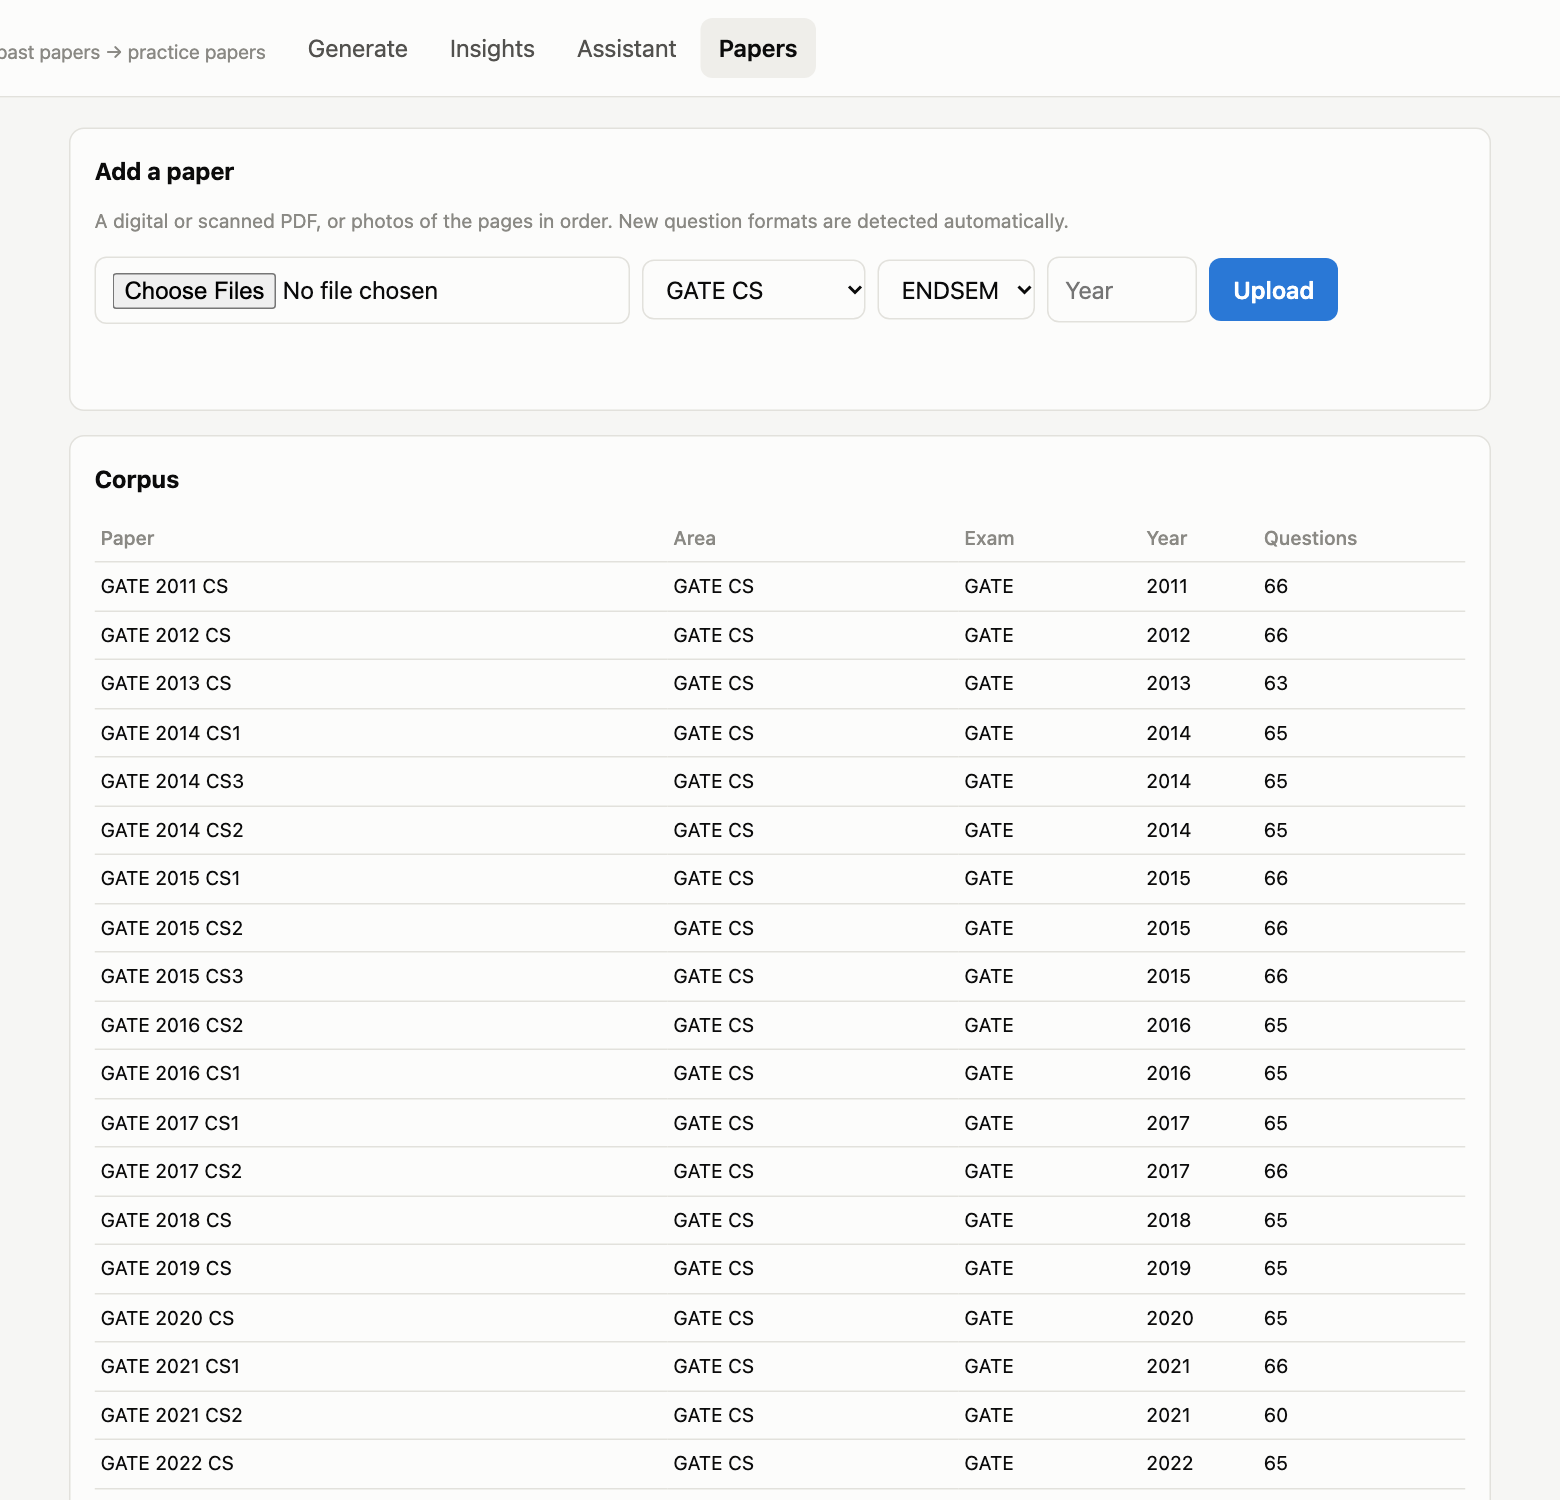
\includegraphics[width=0.9\textwidth]{figures/ui_papers.png}}{}
\caption{Papers tab: corpus listing and upload form for new scanned or digital papers}\end{figure}

\end{document}
